% John L. Godlee (johngodlee@gmail.com)

\documentclass[a4paper, 11pt]{article}
%
\usepackage{amsmath}   % Better maths and more symbols
%
\usepackage{siunitx}
%
\usepackage{geometry}  % Set margins
	\geometry{left=2.2cm,
		right=2.2cm,
		top=2.2cm,
		bottom=2cm}
\parskip 0.5cm
%\twocolumn
%
\usepackage{pdflscape} % Allow landscape pages nested in pdf
%
\usepackage{graphics}  % Insert images easily
\usepackage{graphicx}
\graphicspath{ {img/} }
\usepackage{float}  % Fancy graphics placement [H] [H!] arguments
\usepackage{subfig}
%
\usepackage{caption}
%
\usepackage{enumerate}
%
\usepackage{natbib}    % Bibliography management - Use author/date citations
\bibliographystyle{agsmnourl}  % Use my custom agsm bibliography template which never includes URLs in articles
\usepackage{url}
\usepackage{cite}
%
\usepackage{lineno}
\linenumbers
%
\usepackage{eurosym}
\usepackage{textcomp}
\newcommand{\textapprox}{\raisebox{0.5ex}{\texttildelow}}
%
\usepackage{color} 
\newcommand{\todo}[1]{\textcolor{red}{#1}}   % \todo{NOTE TO SELF WRITTEN IN RED}
%
\title{Geographically and genetically distinct populations of scots pine (\textit{Pinus sylvestris}) differ in resistance to damage by the large pine weevil (\textit{Hylobius abietis}): a common garden translocation study}
\author{John L. Godlee}


%-----------------------------------------------
\begin{document}
%-----------------------------------------------

\maketitle{}

\begin{abstract}

	Damage to coniferous tree plantation crops from the large pine weevil \textit{Hylobius abietis} causes economic losses of \euro{}140 million in Europe \textit{per annum}. Current mitigation strategies are labour intensive and only partially effective. Identifying and breeding natural resistance in host plant cultivars to insect pests has been used in many crop species to reduce damage as part of an integrated pest management strategy. Here, we conducted a common garden experiment in a previously clearfelled forestry plantation where \textit{H. abietis} are known to occur. 672 saplings, grown from seed collected from 21 naturally occurring populations of \textit{Pinus sylvestris} across Scotland were planted together to assess resistance to attack by \textit{H. abietis}.

	On those saplings which were attacked, we found significant variation in the total area of bark lesions between \textit{P. sylvestris} populations. In contrast we found that sapling populations did not differ in their likelihood of being attacked by \textit{H. abietis}. A weak latitudinal pattern was observed, with saplings sourced from populations found further north being attacked more heavily than those further south. From these results it is suggested that as part of an integrated pest management strategy, planting of \textit{P. sylvestris} saplings from more southerly seed-stock may reduce pine weevil attack in affected areas.

% between \textit{P. sylvestris} populations, suggesting that these individuals could be selected for selective breeding to produce trees that are less susceptible to \textit{H. abietis} attack at the sapling stage.

% 26\% of saplings were damaged by \textit{H. abietis} but there was no sapling mortality in the year of the study.

\end{abstract}

\section*{Introduction}

The large pine weevil (\textit{Hylobius abietis} L. Coleoptera: Curculionidae) is a common pest of newly planted coniferous tree plantations in Europe, causing damage to plantation saplings up to around five years old \citep{Ordlander1997}. Adult weevils emerge from tree stumps and feed on the bark and buds of coniferious saplings, consuming sugar rich phloem tissue \citep{Nordlander1991}. Lesions on the bark and buds of saplings (Figure \ref{damage}) as a result of feeding may cause a reduction in growth rate, stem deformation and an increased susceptibility to infection by airborne diseases of trees \citep{Leather1999}. Heavy damage may lead to stem girdling and death of the terminal growing bud resulting in a malformed trunk, limiting economic use as timber when fully grown \citep{Alfaro1989, Gill1992}. While \textit{H. abietis} may inhabit adult coniferous trees in both natural and planted coniferous forests, recently clearfelled and restocked coniferous plantation sites provide an enriched habitat for breeding \textit{H. abietis} and so pose more of a danger to planted saplings than those in naturally regenerating stands \citep{Willoughby2004, Orlander1999}. Adults lay eggs within the stumps of clearfelled trees, which are rarely removed after clearfelling, with newly emerged juvenile weevils feeding on young saplings until adulthood \citep{Willoughby2004}. Planted coniferous saplings are more susceptible to \textit{H. abietis} damage than naturally regenerating saplings, probably due to water stress as a result of damage to root systems during planting \citep{Selander1990}. A single adult weevil can damage several plants over the course of a season, with \textapprox{}50\% sapling mortality observed across affected plantation sites in the UK and Ireland \citep{Heritage2001}. On commercial conifer plantations, \textit{H. abietis} causes annual economic losses of \euro{}140 million \textit{per annum} in Europe, of which \euro{}2.75 million (\textapprox{}\textsterling{}2.47 million) occurs in the UK \citep{Evans2015}. Currently, \textit{H. abietis} is the most damaging insect pest of newly planted trees in Northern Europe \citep{Evans2015}. The potential for climate change to enhance the damage caused by \textit{H. abietis}, by reducing life cycle length \citep{Leather1999} and encouraging migration into previously weevil free areas \citep{Inward2012, Barredo2015}, especially in more northerly regions, has prompted discussion of the effectiveness of current \textit{H. abietis} management practices and possible alternative methods \citep{Kapranas2017, McNamara2018}.

\begin{figure}[H]
\centering
	\subfloat[]{
		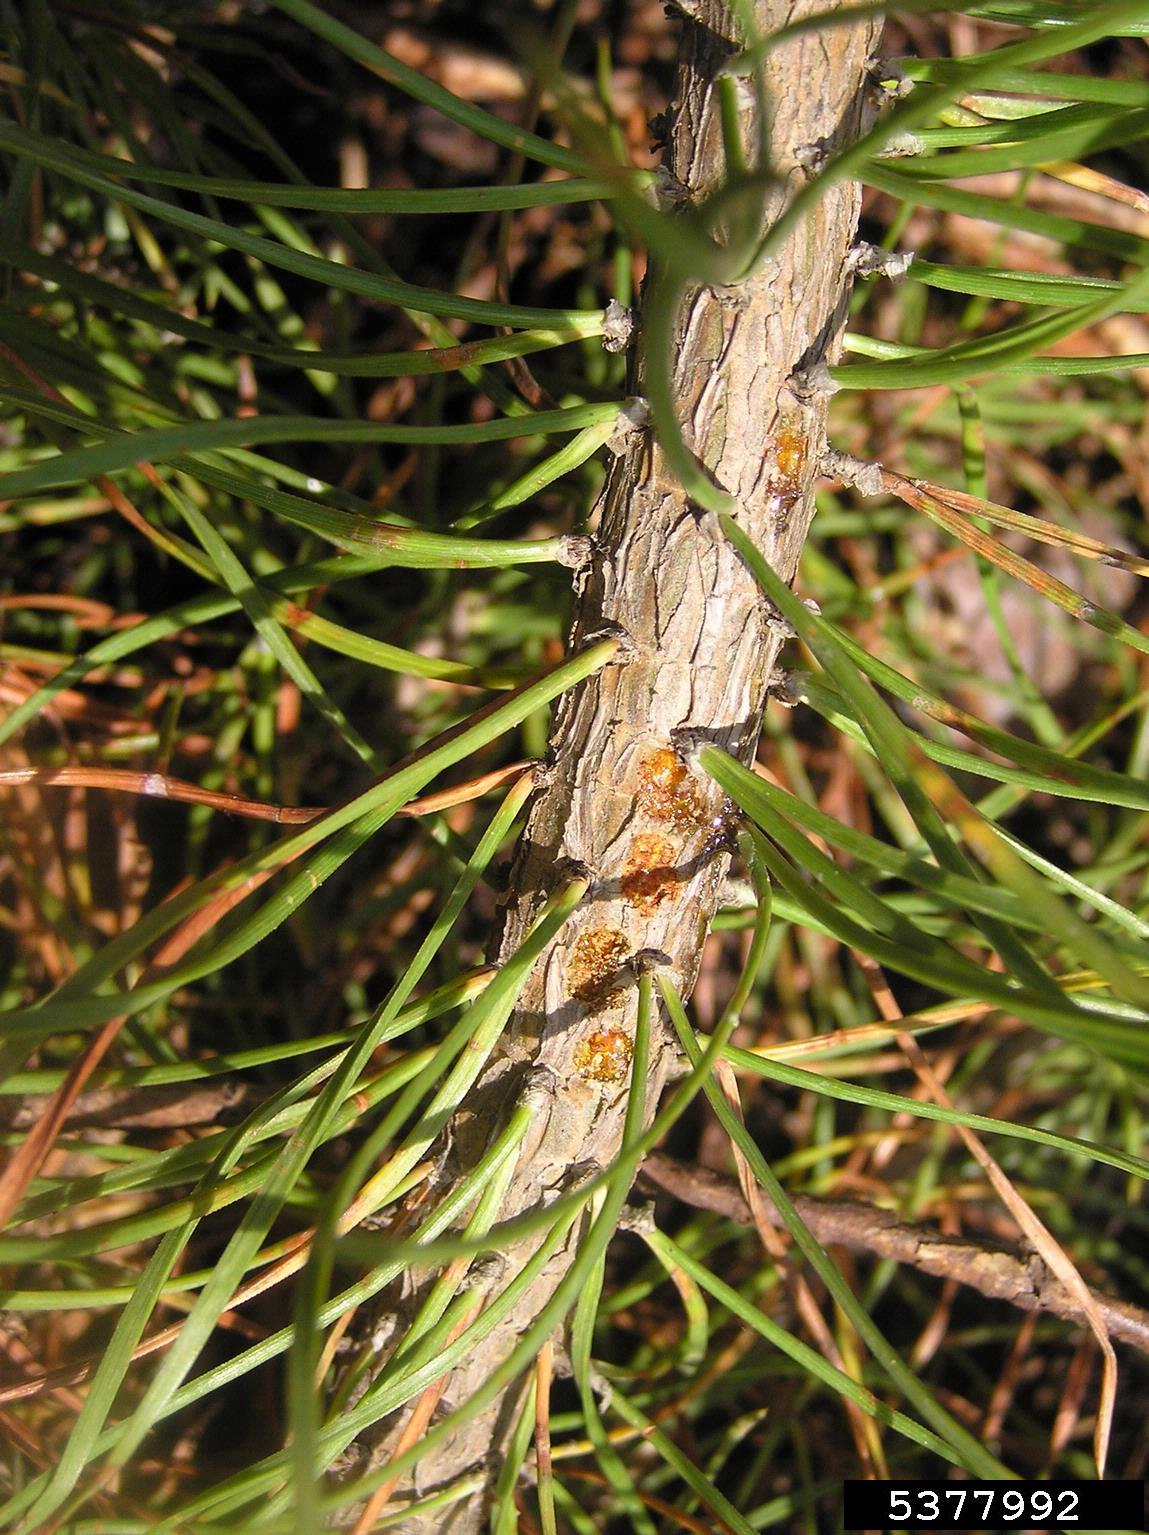
\includegraphics[width=0.4\textwidth]{damage_low} 
	}
	\subfloat[]{
		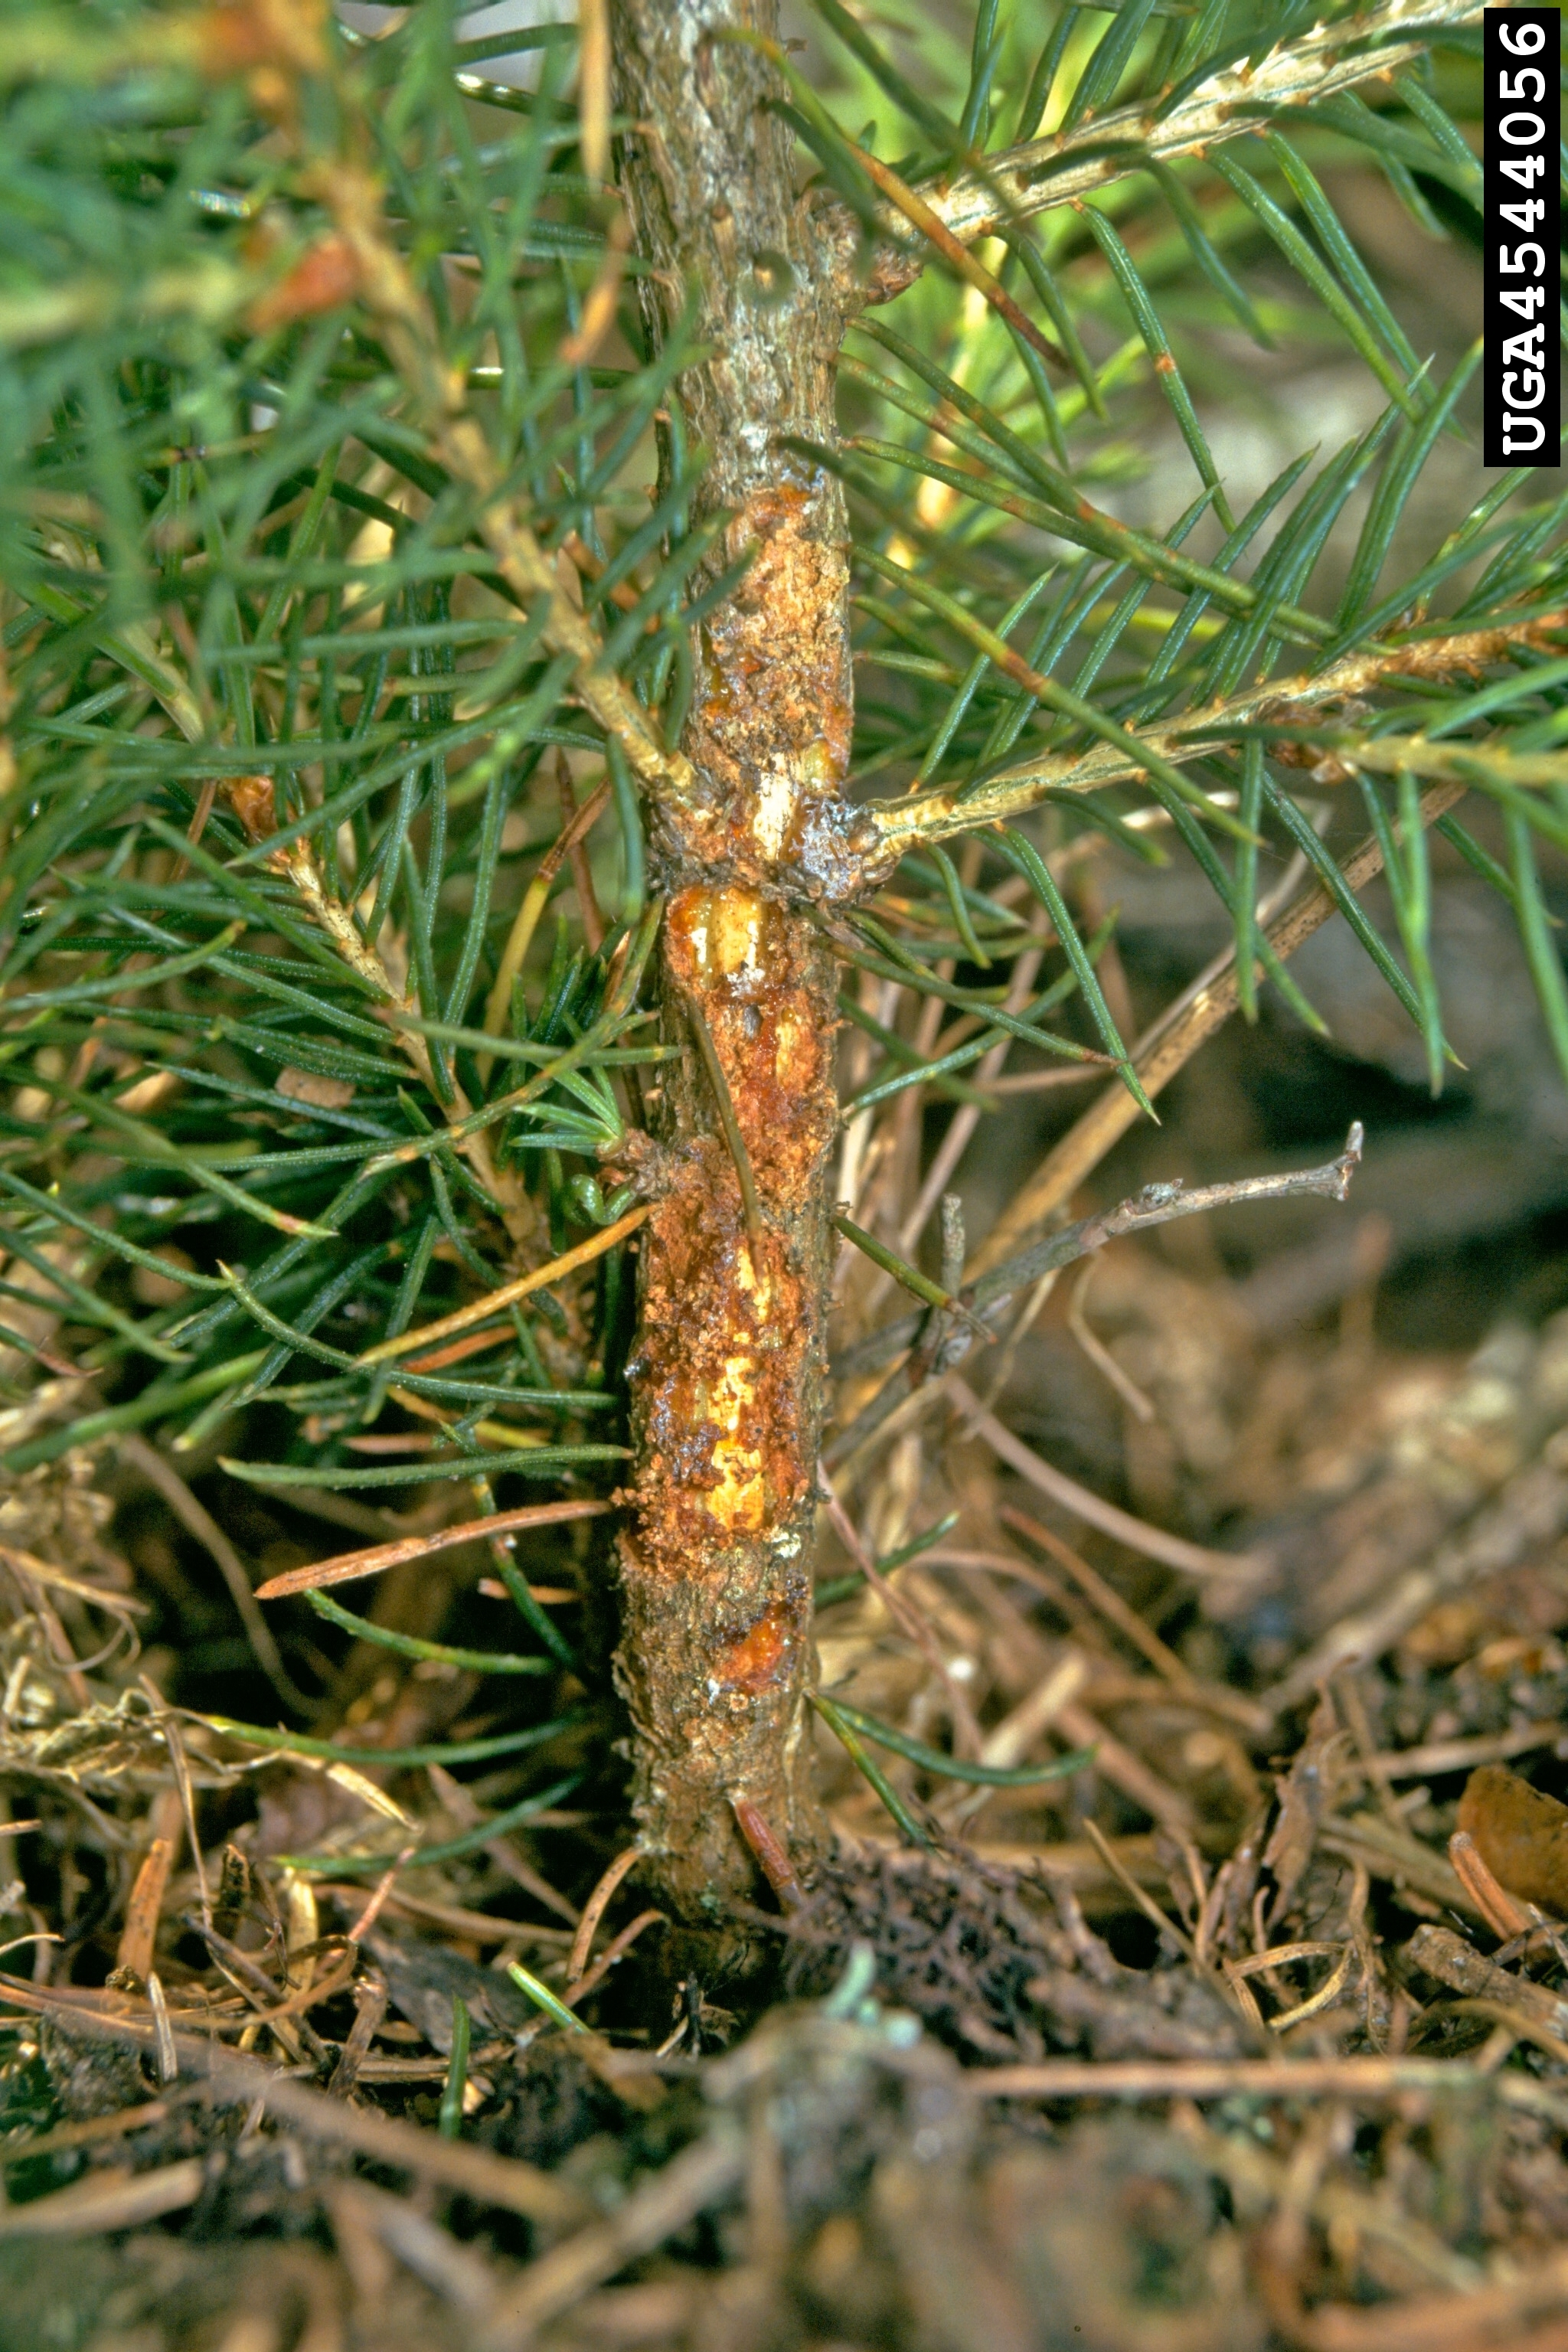
\includegraphics[width=0.4\textwidth]{damage_high}
	}
	\caption{Damage caused by \textit{Hylobius abietis}, destroying phloem tissue and causing scarring of the stem. (a) shows light damage with individual circular lesions, while (b) shows heavier damage with exposure of wood beneath the bark. Images taken from (a) Milan Zubrik, Forest Research Institute - Slovakia, Bugwood.org, and (b) Petr Kapitola, Central Institute for Supervising and Testing in Agriculture, Bugwood.org.}
	\label{damage}
% https://www.forestryimages.org/browse/detail.cfm?imgnum=4544056
% https://www.forestryimages.org/browse/detail.cfm?imgnum=5377992
\end{figure}

Management of \textit{H. abietis} currently relies on a variety of chemical, biological and physical measures, with integrated pest management schemes tending to yield greater success \citep{Willoughby2004}. Physical deterrents include piling debris produced by the clearfelling process over exposed stumps to discourage egg laying \citep{Rahman2015}, or stump removal to limit the availability of substrate for egg laying. The application of entomopathogenic nematodes after clearfelling has been shown to reduce the number of adult weevils in clearfelled sites \citep{Dillon2006, Kapranas2017, Williams2013}. The most common method of control is the addition of chemicals at the time of restocking, with \textit{H. abietis} being the only insect pest against which routine chemical controls are applied in the UK and Ireland \citep{Willoughby2004, Willoughby2017}. The most common chemical application for \textit{H. abietis} in the UK are syntehtic pyrethroids of various formulation, which are sprayed directly onto saplings as a prophylactic treatment, acting as a strong deterrent for \textit{H. abietis} feeding on treated bark \citep{Rose2005}. There are concerns however about run-off from spraying events entering watercourses, where it is highly toxic to aquatic organisms \citep{Willoughby2017, Mian1992, Antwi2015}. There are also concerns about the health of forestry workers who apply the sprays \citep{Rose2002}. Additionally, the application of pyrethroid sprays can cost \textapprox{}\textsterling{}80 per hectare of planted land, and requires additional top-up sprays in subsequent years if the problem persists during the sapling stage \citep{Willoughby2017}.  

\textit{H. abietis} adults rely on olfaction to search for coniferous hosts, responding to Volatile Organic Compounds (VOCs), dominated by $\alpha$-pinene and other monoterpenes released by the host plant \citep{Nordlander1986, Nordlander1987}. At the local scale, when adult \textit{H. abietis} are searching for feeding material while on the ground, after their flight muscles regress, VOCs released by open wounds on the bark caused by previous pine weevil feeders may attract more individuals \citep{Nordlander1987, Tilles1986}, worsening the damage caused to the sapling. A positive feedback mechanism may therefore exist, whereby damaged saplings are more likely to be further damaged, acting as beacons for other \textit{H. abietis} individuals. Conifer saplings may also use VOCs as a defensive strategy however, to deter insect pests \citep{Gershenzon1991, Trapp2001}. Conifer saplings may differ in the concentration of VOCs produced both prior to damage and after bark has been damaged by feeding \citep{Kivimaenpaa2012, Keeling2006}, and in their chemical composition \citep{Heijari2011} potentially causing variation in the likelihood of a sapling becoming damaged by \textit{H. abietis}. Other defensive strategies employed by coniferous tree species against insect herbivores include higher concentrations of sclereid cells in the bark and resin canals in the needles, making the plant material less palatable to herbivores, thus deterring continued feeding \citep{Donnelly2016, King2011}.

While \textit{H. abietis} is a generalist of a number of coniferous tree species \citep{Wallertz2014, Toivonen2006}, they are common pests in scots pine (\textit{Pinus sylvestris} L. Pinaceae) plantations \citep{Manlove1997}. An increasing percentage of coniferous plantation forestry in the UK is \textit{P. sylvestris}. It currently constitutes \textapprox{}17\% of the UK's commercial coniferous plantation forestry by area and \textapprox{}15\% by biomass \citep{ForestryStatistics2018}. It is one of the UK's three native coniferous tree species \citep{Cheffings2005}. There is increasing interest to plant native tree species in an attempt to preserve native biodiversity and landscape heritage \citep{}. \textit{H. abietis} is the most serious pest of UK \textit{P. sylvestris} plantations, with infestations sometimes precluding sustainable future planting completely due to sapling mortality on clearfell sites \citep{Willoughby2017}.

Selective breeding and identification of \textit{P. sylvestris} varieties that are resistant to \textit{H. abietis} attack may provide a low cost method to reduce damage to saplings. Resistant varieties could form part of an integrated pest management scheme \citep{Telford2014} and planting of multiple varieties in a single forest patch could act as good insurance against potential future attacks in a rapidly changing pest landscape due to climate change \citep{Alfaro2014}. Indeed, selecting for and inducing natural resistance to \textit{H. abietis} and other bark boring insects is being heavily explored with other coniferous tree species such as \textit{Picea abies} (Norway spruce) \citep{Eyles2009, Schiebe2012}, \textit{Picea sitchensis} (Sitka spruce) \citep{King2011}, and \textit{Picea glauca} (white spruce) \citep{Kiss1991}, but \textit{P. sylvestris} has not recieved the same attention. \citet{Byun2006} found that \textit{P. sitchensis} populations varied in their expression of genes responsible for the production of bark oleoresin ducts when saplings were damaged, which act as a defence against stem boring insects. Similarly, \citet{Alfaro2013} developed varieties of \textit{P. sitchensis} resistant to the white pine weevil (\textit{Pissodes strobi} Peck Coleoptera: Curculionidae). They concluded that resin canals and sclereid cells in the bark as well as terpene production and variation in tree phenology were heritable characteristics which confer resistance to attack by \textit{P. strobi}.

Natural populations \textit{P. sylvestris} are restricted to enclaves in the north of Scotland. Remnant Caledonian pine populations in Scotland, where \textit{P. sylvestris} is the dominant species \citep{Edwards2006} are comprised of 84 fragmented woodland stands dominated by \textit{P. sylvestris}, over a total area of 17,882 hectares \citep{Mason2004}, which maintain adaptive genetic variation. Previous studies have shown that these populations vary in their ability to tolerate pathogens \citep{Perry2016} and environmental extremes \citep{Salmela2013}. This study contributes further by assessing the tolerance of natural \textit{P. sylvestris} populations to \textit{H. abietis} attack, with the hope of informing future selection of pine weevil resistant \textit{P. sylvestris} cultivars for plantation forestry, and identifying potential future conservation concerns for naturally occurring \textit{P. sylvestris} in Caledonian remnant forests. 

We conducted a common garden experiment in a recently clearfelled plantation already affected by \textit{H. abietis} with \textit{P. sylvestris} saplings in southern Scotland to assess sapling resistance to damage from the large pine weevil \textit{H. abietis}. We compared germinated seedstock collected in naturally occurring \textit{P. sylvestris} populations in remnant Caledonian pine forest patches across Scotland (Figure \ref{site_map}). We hypothesised that due to limited gene flow between Caledonian pine remnants, adaptive variation in attractiveness to \textit{H. abietis} as a food source would exist between populations of \textit{P. sylvestris}. We hypothesised that two effects contribute to the extent of damage which a sapling is subject to, based on the previous work discussed above regarding \textit{H. abietis} host searching behaviour: the probability of \textit{H. abietis} initially choosing to feed on a sapling and damaging its bark (a), and the intensity of continued feeding by \textit{H. abietis} (b). 

\section*{Materials \& Methods}

\subsection*{Study sites and species}

Scots pine (\textit{Pinus sylvestris}) is the most widely distributed pine species in the world. It's range spans Eurasia from the arctic circle in Scandinavia to the dry northern mediterranean in Spain and Turkey and from Scotland to the eastern edge of Siberia \citep{GBIF2019, Carlisle1968}. Scotland represents the western limit of its Eurasian distribution, where it is the dominant canopy tree species of the Caledonian pine forest. \textit{P. sylvestris} grows well under conditions of low grazing, shade and competition. 

\textit{P. sylvestris} is wind pollinated, with monoecious flowering beginning between the ages of 15 and 30. Previous studies have shown cryptic genetic variation between the Caledonian remnant forest sites from which seeds used in this study are sourced \citep{Donnelly2018}, which supports the assertion that despite strong cross-pollination effects between the populations, some degree of genetic isolation occurs. Variation in isolatedness between sites follows a predictable longitudinal gradient, with sites on the western extreme of the Caledonian pine range being more isolated due to the prevailing easterly wind direction limiting pollen dispersion to the west \citep{Gonzalez2018}. 

Seed populations of \textit{P. sylvestris} were collected from 21 sites where genetic variation has already been identified across Scotland in March 2007 (Figure \ref{site_map}). At each site four open-pollinated trees were located at least 100 m apart. From each of these trees at least 20 cones with seeds were collected. To minimise seedling mortality, seeds were germinated and grown in a glasshouse for 3 years before four randomly selected surviving seedlings per Parent tree were transplanted to a common garden. This resulted in 168 distinct maternal lines. All seed was collected from old adult trees, in an attempt to avoid sampling trees descended from nearby plantation forestry as this study focussed only on natural populations. Sites were situated within the historical range of the Caledonian pine forest. Seed collection sites were chosen by accessibility in six geographic clusters. Each cluster was located to ensure geographical isolation from others. 

\begin{figure}[H]
	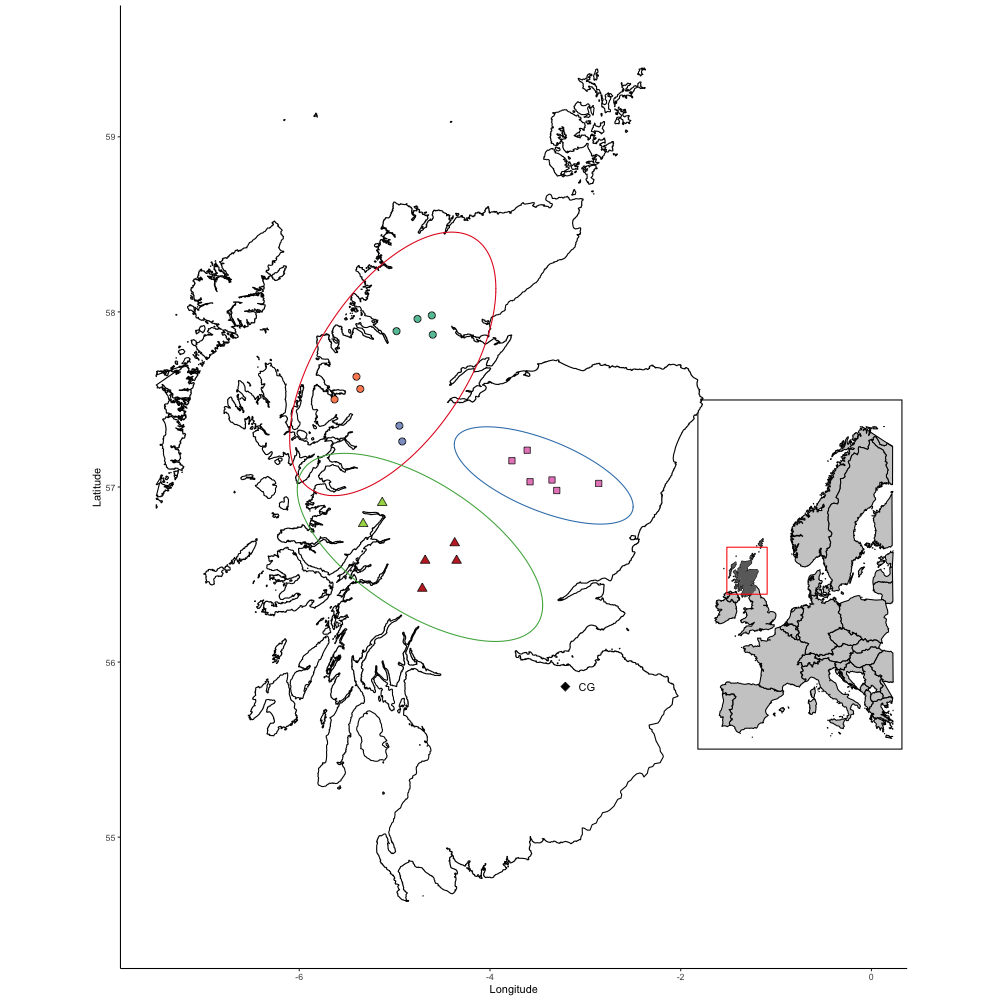
\includegraphics[width=\textwidth]{site_map}
	\caption{Map of seed collection sites within Scotland, from which seed populations were collected. Elliptic hulls and site point shapes define the three Regions. Points are coloured according to Geographic Zone clusters, which are nested within Regions. Point labels are Site codes used as a shorthand for the sites throughout this report.} 
	\label{site_map}
\end{figure}

\subsection*{Experimental design}

The common garden was located in Southern Scotland (N 55.86\textdegree{}, E \textminus{}3.21\textdegree{}) in a patch of recently clear-felled sitka spruce (\textit{Picea sitchensis}) plantation, surrounded by existing adult \textit{P. sitchensis} plantation on all sides. This mimicks the conditions found in commercial plantation forestry sites that will be replanted, which often have adjacent existing plantation. A mown grass border of 10 m on all sides separated the newly planted \textit{P. sylvestris} from the surrounding \textit{P. sitchensis} plantation, to avoid competitive edge effects. All \textit{P. sitchensis} surrounding the common garden was planted at the same time in 2005, making it 10 years old when the common garden was established. %Planting was divided into four blocks of equal size running perpendicular to the average slope of the site. Each block contained 167 saplings, with saplings placed in a grid pattern within each block, with a gap between each sapling of \todo{METRES} and between saplings and the plot edge \todo{FIGURE REF}. 
Saplings were randomly assigned to grid points within 4 adjacent blocks with a distance of 3 m between each sapling. This resulted in a total grid size of 84 x 8 saplings, a total of 672 saplings. \textit{H. abietis} infestation occurred naturally across the site, with adult weevils likely travelling from the adult \textit{P. sitchensis} plantation around the common garden. 

\subsection*{Data collection}

The area of bark lesions caused by \textit{H. abietis} was measured on the main growing stem of each sapling in June 2015. This is roughly between the two seasonal peaks of weevil feeding that are commonly observed in the UK, which occur in the spring and late summer, coinciding with the end of adult hibernation and the emergence of new adults from pupae, respectively \citep{Nordenhem1989, Leather1999}. Only damage sustained by \textit{H. abietis} during the current growing season was counted and could be clearly separated from damage sustained in previous years by the lack of bark edge scarring and presence of sap at the wound edge (Figure \ref{damage}). Isolated lesions tended to be roughly circular with a diameter of \textapprox{}3 mm. Where a larger continuous lesion was found, as when a stem was girdled, the larger lesion was photographed with a scale and the area estimated by tracing the lesion with ImageJ version 1.50g7 \citep{Schneider2012}. Weevil damage is therefore expressed as the mm\textsuperscript{2} area of stem lesions per sapling. 

\subsection*{Statistical analysis}

To assess the effect of \textit{P. sylvestris} sapling genetic origin on damage by pine weevils (\textit{H. abietis}), and to test our hypothesis that two effects are responsible for \textit{H. abietis} damage, we implemented a hurdle model framework with generalised linear mixed models, using the \textit{glmmTMB} package in R \citep{glmmTMB}. First, a binomial logistic mixed effects model assessed variation in the probability of a sapling being initially damaged  according to \textit{P. sylvestris} Site.

We used a linear mixed effects model, using only saplings where damage had occurred, to assess whether saplings varied in the total area of bark damaged by continued feeding by \textit{H. abietis} according to \textit{P. sylvestris} Site. The response variable of area of bark damaged was log transformed in order to better meet model assumptions. In both analyses, a combination of fixed and random intercept effects were modelled to obtain the optimal model structure and to compare the relative effect sizes of Geographic Zone, Site and Parent tree. Parent tree was used as a random intercept effect in all analyses to account for pseudo-replication in sapling Parent. The geographically nested nature of the seed collection Sites within Geographic Zones was also used as a random effect in the appropriate models (Figure \ref{dendro}). Model goodness-of-fit was assessed for both model types by comparing models with equivalent random effects models and null models using AIC\textsubscript{r} (Akaike Information Criterion) and Log-likelihood estimates \citep{Bolker2008}. During model comparison all models were fitted using Maximum Likelihood (ML) \citep{Bolker2008}. To investigate which populations of \textit{P. sylvestris} differed in their resistance to \textit{H. abietis} attack, the models were refitted using Restricted Maximum Likelihood (REML) and model slope estimates were compared. Tukey's HSD multiple comparisons tests of marginal means assessed which populations were significantly different from each other for both models, using the \textit{emmeans} package \citep{Russell2019}. All statistical analyses were performed in R version 3.4.2 \citep{RCoreTeam2019}. 

A post-hoc linear mixed effects model investigated the effect of latitude of seed collection Site on the area of damaged bark, with nested random intercept effects of Parent within Site. Predicted values of this model were generated and used to assess the effect of latitude on damaged bark area. 

Spatial autocorrelation may have been present within the Common Garden, with some damaged saplings acting as olfactory beacons to attract more\textit{H. abietis} to the area. This potential effect was investigated using Generalised Least Squares (GLS) models of damaged bark area with spatial autocorrelation structures as a covariate. Multiple spatial autocorrelation structures were tested and models fitted using ML were compared in their goodness-of-fit using AIC (Akaike Information Criterion) values, Log-likelihood estimates and pseudo R-squared model values calculated by the \textit{MuMIn} package \citep{MuMIn}. After model selection, the best generalised least squares model was re-fitted using REML for model interpretation to assess the predictive effect of spatial auto-correlation on weevil damage. Along with the GLS model effect size, semi-variograms of the raw damaged area mm\textsuperscript{2} data confirmed that spatial autocorrelation between saplings was negligible within the Common Garden and so spatial autocorrelation structures were not included in other models.

\section*{Results}

\subsection*{Sapling damage}

36.9\% (248/672) of the saplings in the common garden were damaged by \textit{H. abietis} feeding activity. Figure \ref{barchart} shows the number of saplings damaged divided into their origin seed collection Sites. All saplings were alive prior to data collection and sapling mortality was not recorded during the experiment. All seed populations had at least eight affected saplings out of a total of 32. The population with the highest number of damaged saplings was Loch Clair (LC), which had 18 damaged saplings. The sapling with the highest mm\textsuperscript{2} damaged area was from Cona Glen (CG) and had 325.8 mm\textsuperscript{2} of bark damaged. Rhidorroch (RD) had the highest cumulative damaged area with 1057.1 mm\textsuperscript{2}. Variation in bark area damaged within seed populations was high (Figure \ref{boxplot}), with some geographic zones having similar levels of damage while others varied a widely within geographic zone.

\begin{figure}[H]
	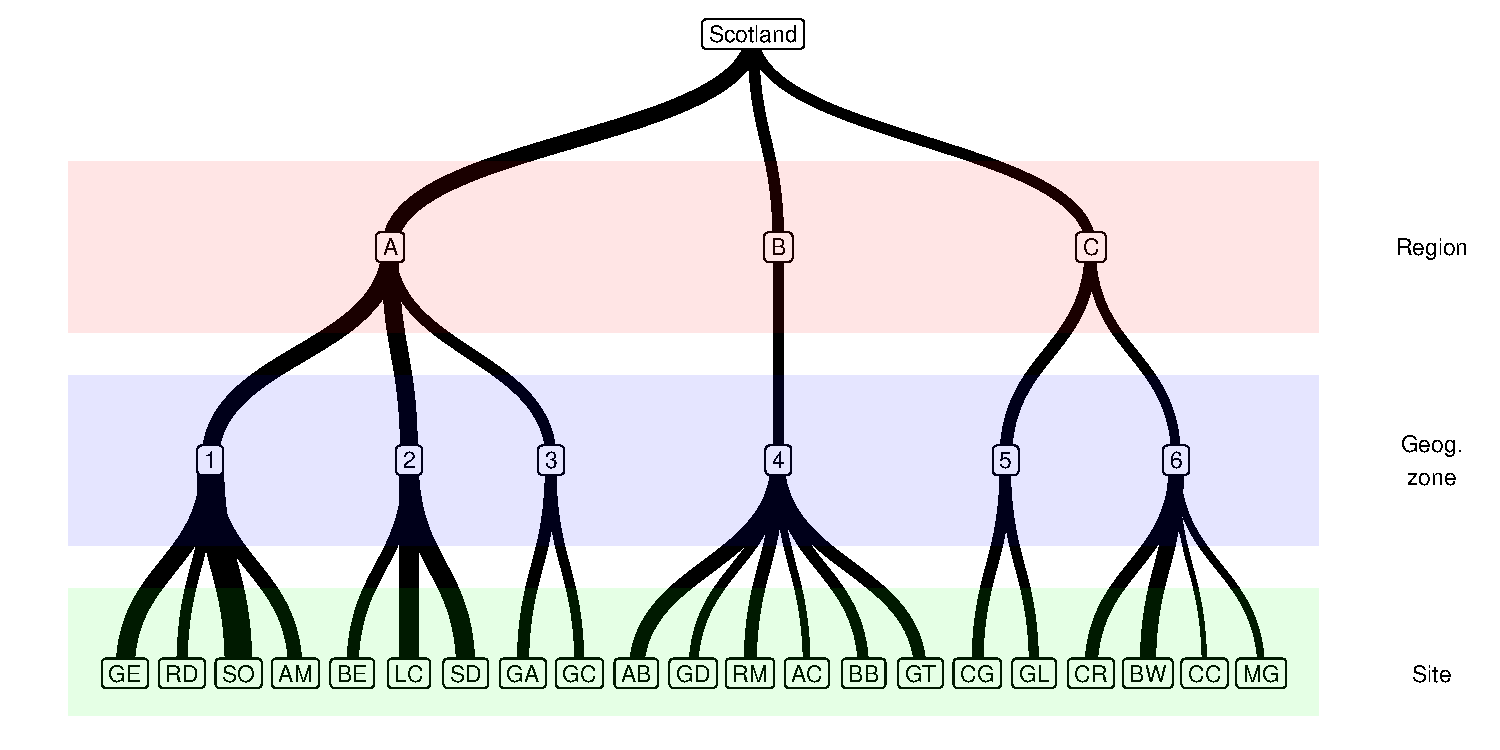
\includegraphics[width=\textwidth]{dendro}
	\caption{Dendrogram showing nested grouping of seed populations. Graph edge widths vary relatively according to the total bark area damaged on saplings collected from each Site. Width edges are weighted according to the number of saplings at each grouping level to account for differences in number of Sites per Geographic Zone and Region. This means edge widths should not be compared across vertical node levels.}
	\label{dendro}
\end{figure}

\begin{figure}[H]
	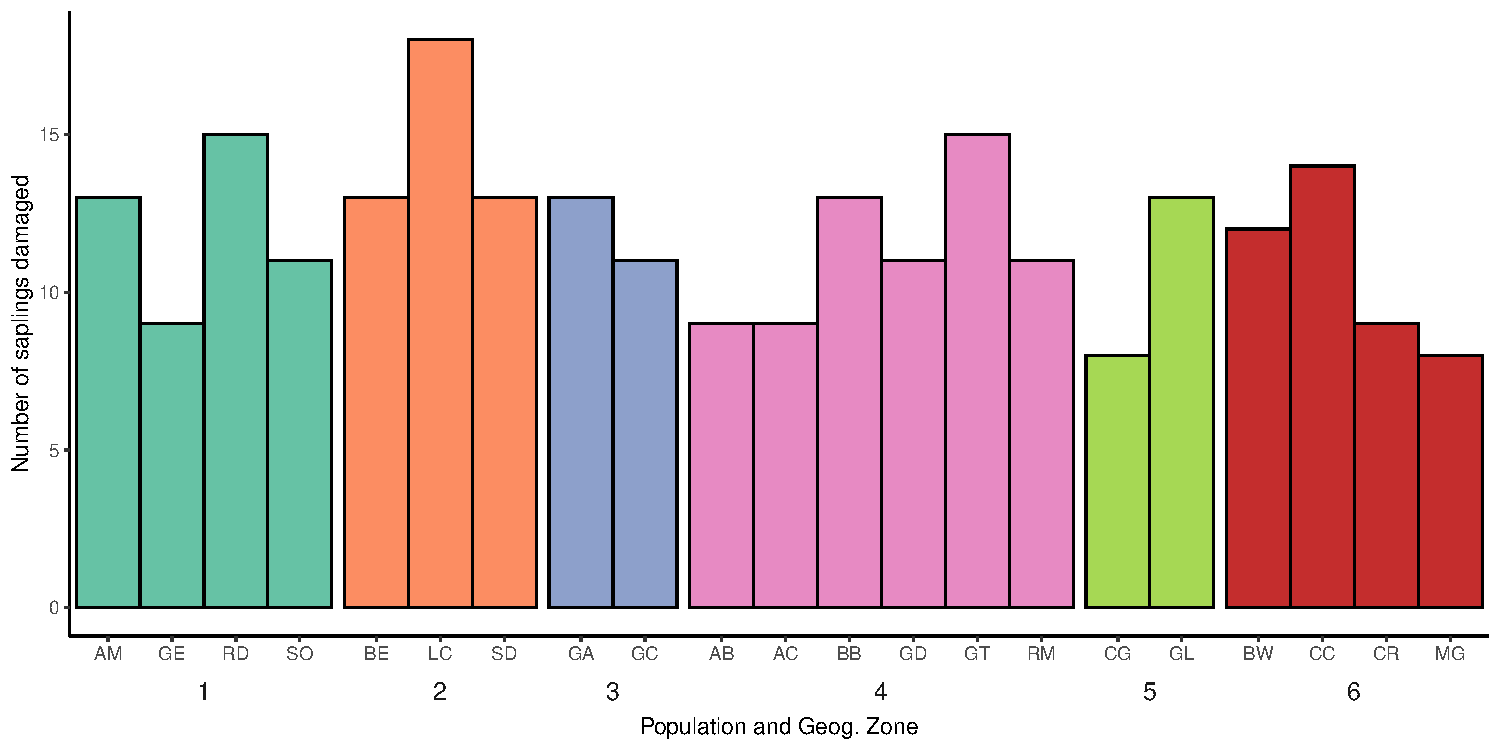
\includegraphics[width=\textwidth]{barchart}
	\caption{The number of saplings with visible damage by \textit{H. abietis}, divided by Site. Groups of bars denote Geographic Zones.}
	\label{barchart}
\end{figure}

\begin{figure}[H]
	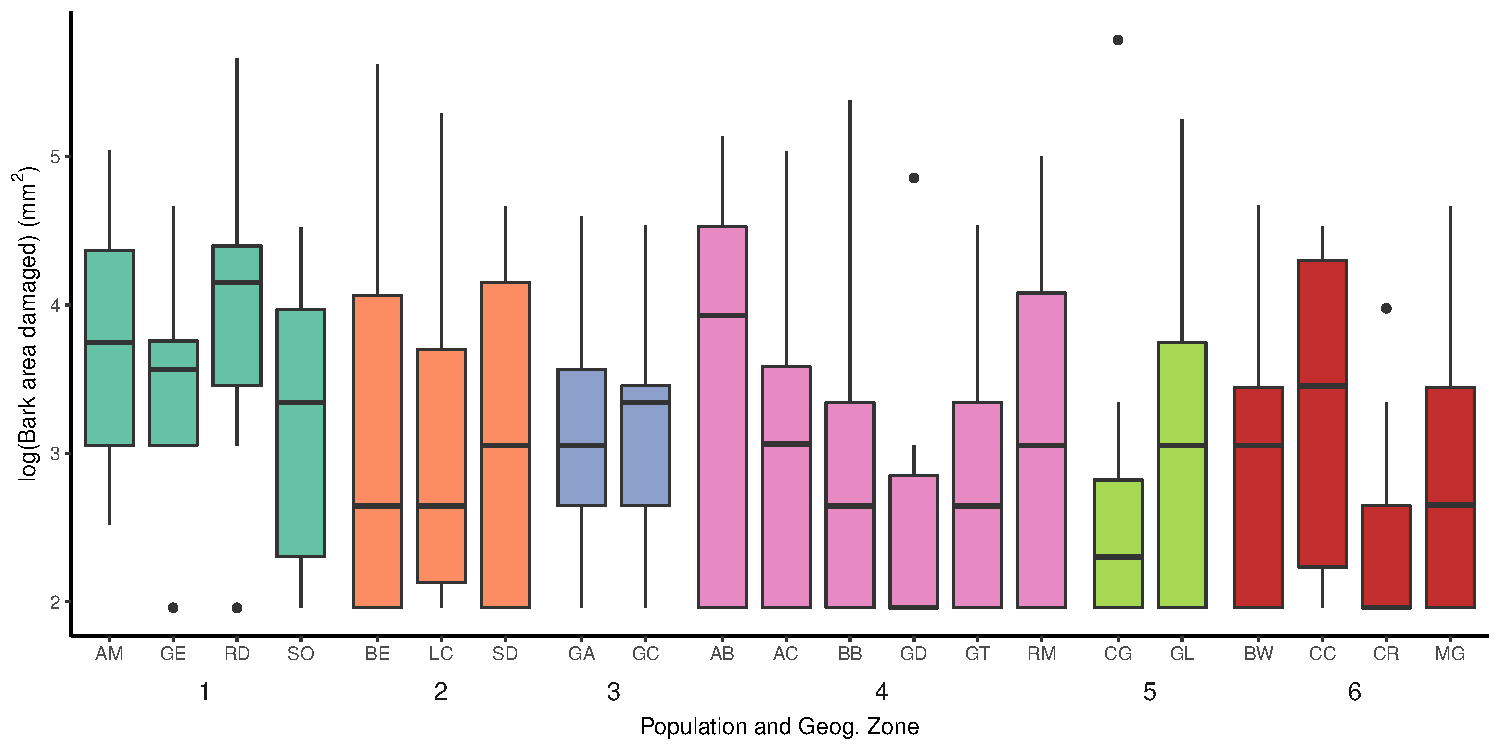
\includegraphics[width=\textwidth]{boxplot}
	\caption{Variation in bark area damaged by \textit{H. abietis}, divided by Site. Coloured groups of bars denote Geographic Zones. Thick bars denote the median value per population.}
	\label{boxplot}
\end{figure}


\subsection*{Spatial auto-correlation}

Multiple Generalised Least Squares (GLS) models of damaged sapling area fitted with different correlation structures were compared against a null model with no correlation structure using AIC values (Table \ref{cor_table}). A Gaussian correlation structure fit the data best, but explained only a very low percentage of the variation in sapling damaged area. Gaussian, Exponential and Rational quadratic models had AIC values within 2 points of each other and explained only negligibly different amounts of variation in damaged bar area, according to pseudo-R\textsuperscript{2} model values, so these models can be interpreted as fitting the data similarly well. All three models were better than a null model which explained none of the variation in damaged bark area. A semivariogram of damaged bark area with distance between saplings showed that there was no appreciable spatial auto-correlation, with all adjacent sapling distances occurring after the nugget of the semivariogram (Figure \ref{semivariogram}). This was supported by a visual inspection of a schematic map of damaged bark area per sapling in the common garden (Figure \ref{sapling_map}). As a result, further modelling with mixed effects models did not include a spatial auto-correlation covariate structure.

\begin{figure}[H]
	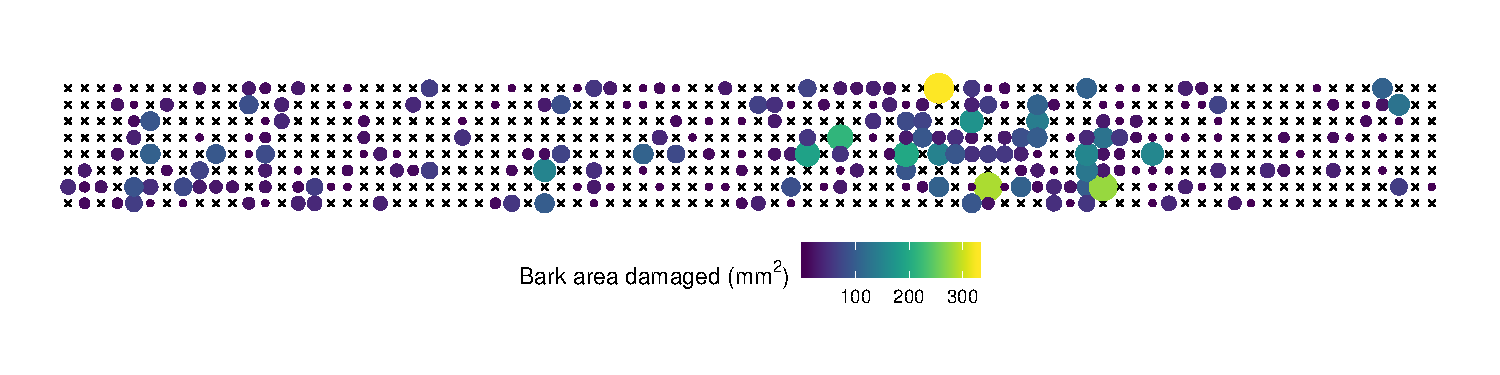
\includegraphics[width=\textwidth]{sapling_map}
	\caption{Schematic diagram of sapling relative position within the Common Garden, with sapling points coloured and sized according to the area of bark damaged. The distance between saplings is 3 m in both the X and Y directions.}
	\label{sapling_map}
\end{figure}

\begin{figure}[H]
	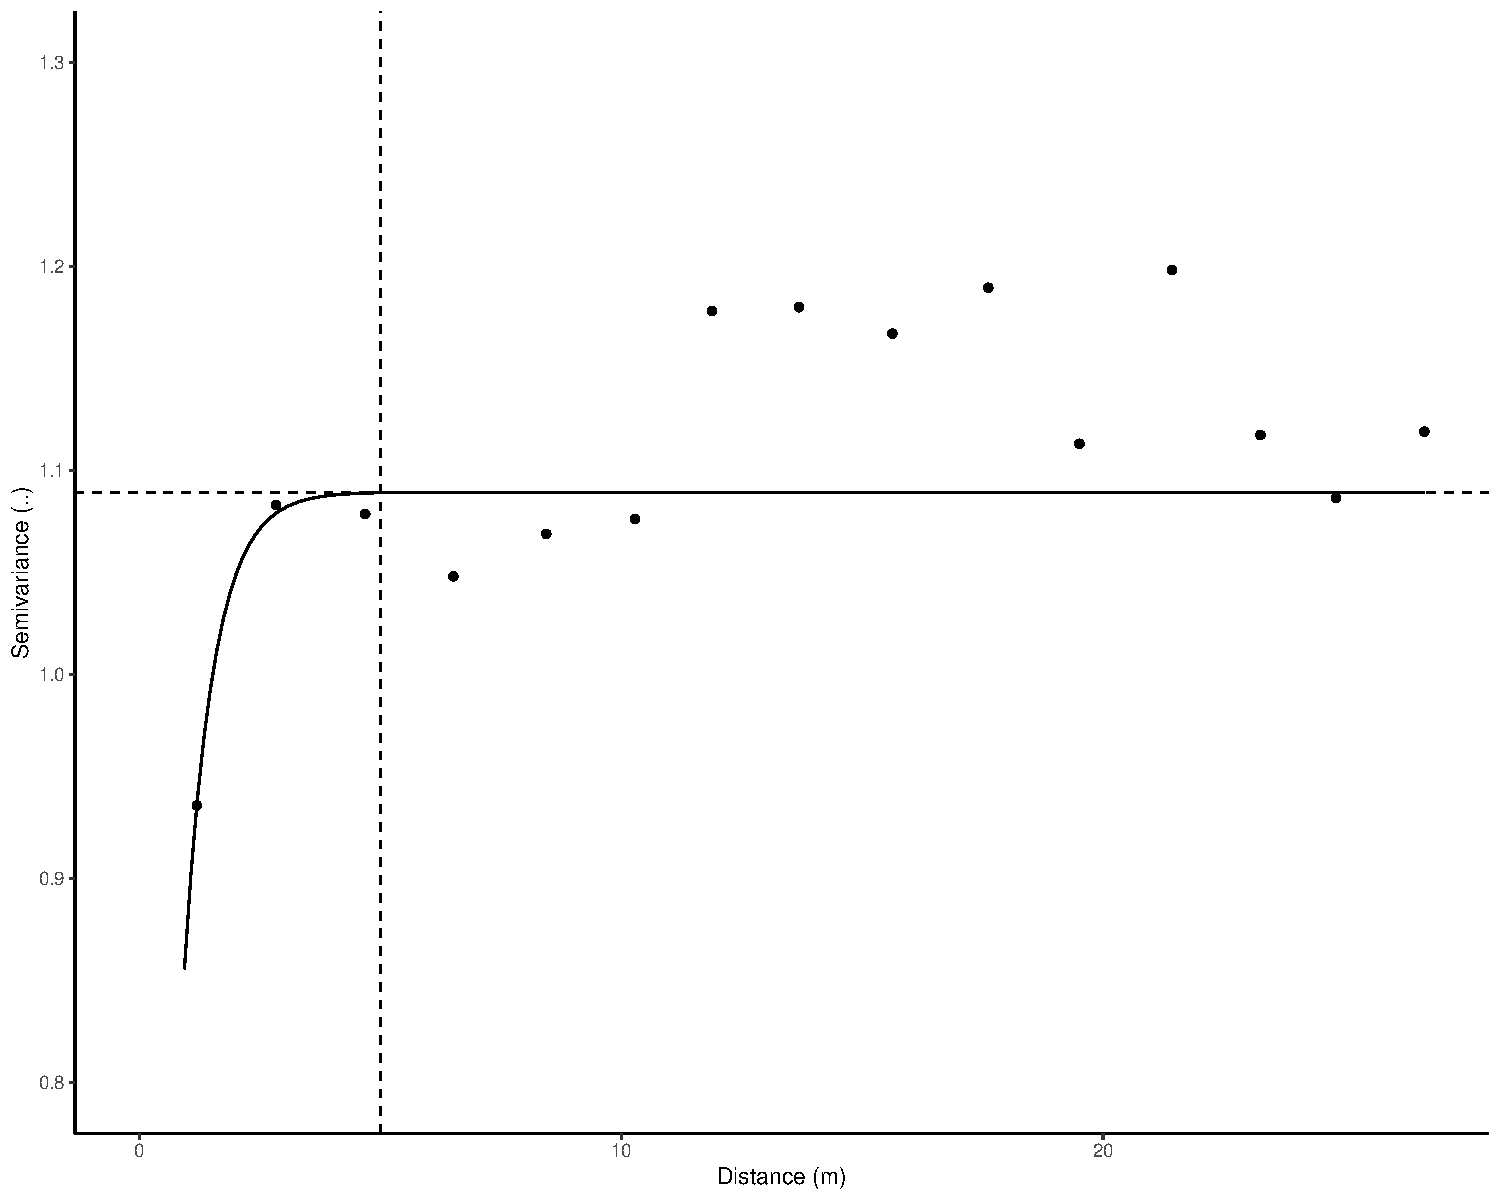
\includegraphics[width=\textwidth]{variogram}
	\caption{Semivariogram showing spatial autocorrelation of damaged bark area according to distance between saplings. Vertical dotted line denotes the nugget and the horizontal dotted line denotes the sill of the semivariogram.}
	\label{semivariogram}
\end{figure}


% Table created by stargazer v.5.2.2 by Marek Hlavac, Harvard University. E-mail: hlavac at fas.harvard.edu
% Date and time: Tue, Aug 06, 2019 - 09:04:03
\begin{table}[H] \centering 
  \caption{Model comparison of Generalised Least Squares models predicting damaged sapling bark area using different spatial autocorrelation structures. Models are ordered by increasing AIC value.} 
  \label{cor_table} 
\begin{tabular}{@{\extracolsep{5pt}} lS[table-format=3.2]S[table-format=3.2]S[table-format=3.2]} 
\\[-1.8ex]\hline 
\hline \\[-1.8ex] 
{Cor. Struct.} & {AIC} & {logLik} & {R\textsuperscript{2}\textsubscript{m}} \\
\hline \\[-1.8ex] 
Gaussian & 719.573 & -355.786 & 0.033 \\ 
Exponential & 720.306 & -356.153 & 0.031 \\ 
Rational quadratic & 720.496 & -356.248 & 0.028 \\ 
Null & 725.404 & -360.702 & -0 \\ 
Spherical & 728.224 & -360.112 & 0.004 \\ 
Linear & 728.224 & -360.112 & 0.004 \\ 
\hline \\[-1.8ex] 
\end{tabular} 
\end{table} 


\subsection*{The effect of seed population on sapling damage}

\subsubsection*{Binomial model}

The first part of the hurdle model process explored variation among seed populations in the probability of a sapling being damaged by \textit{H. abietis}. The most parsimonous model was a null model, as estimated by AIC values. Fixed effects models using Geographic Zone and Site explained little of the variance in likelihood of a sapling being damaged, while models using Parent as the fixed effect explained \textapprox{}95\% (R\textsuperscript{2}\textsubscript{m} of the variance (Table \ref{binom_comp}). Parent models were the least parsimonious however, with $\Delta$AIC values of 147.73 and 145.73. The fixed effect of Parent accounted for most of the model variance for those models (R\textsuperscript{2}\textsubscript{c} = \textapprox{}94\%), however a pairwise comparison of marginal means for each family revealed that none differed significantly from each other, indicating the model is likely overfitted due to the large number of Parent groups. We compared marginal means of the fixed effect groups for the best fitting models using Geographic Zone or Site as fixed effects and found that these groups did not vary significantly in a pairwise comparison (Figure \ref{binom_margin}a,b).

\begin{figure}[H]
\centering
	\subfloat[]{
		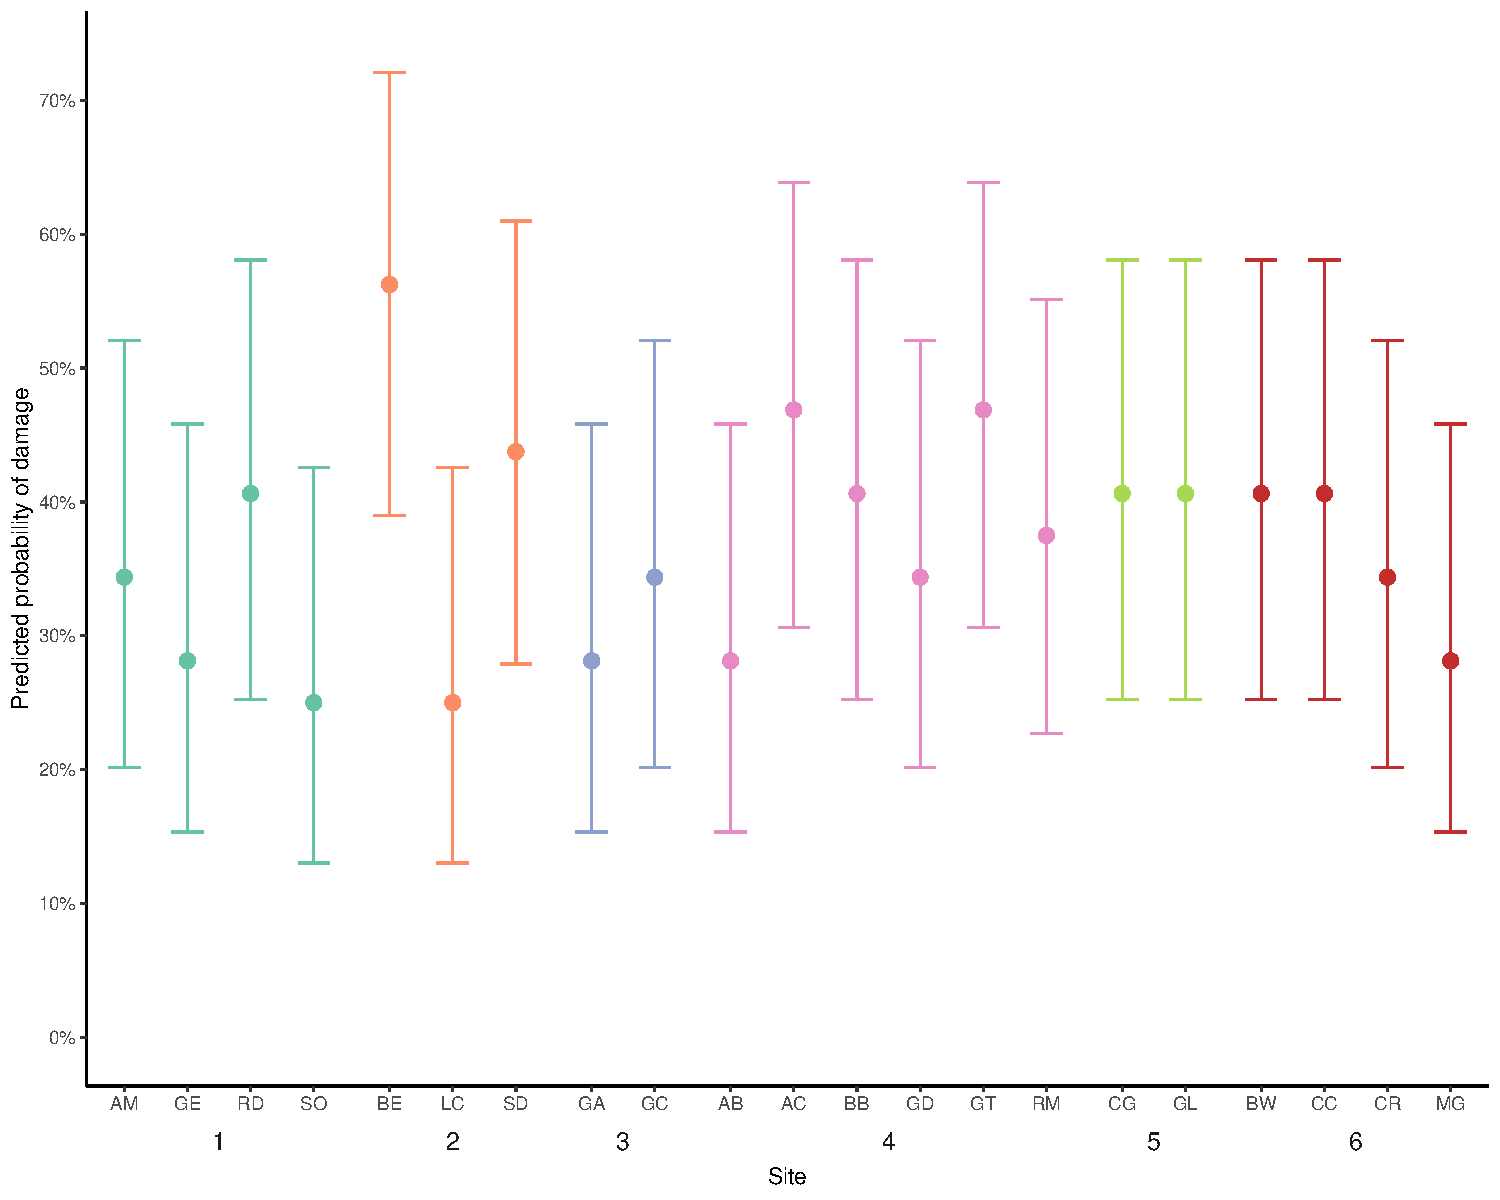
\includegraphics[width=0.5\textwidth]{pred_binom_site}
	}
	\subfloat[]{
		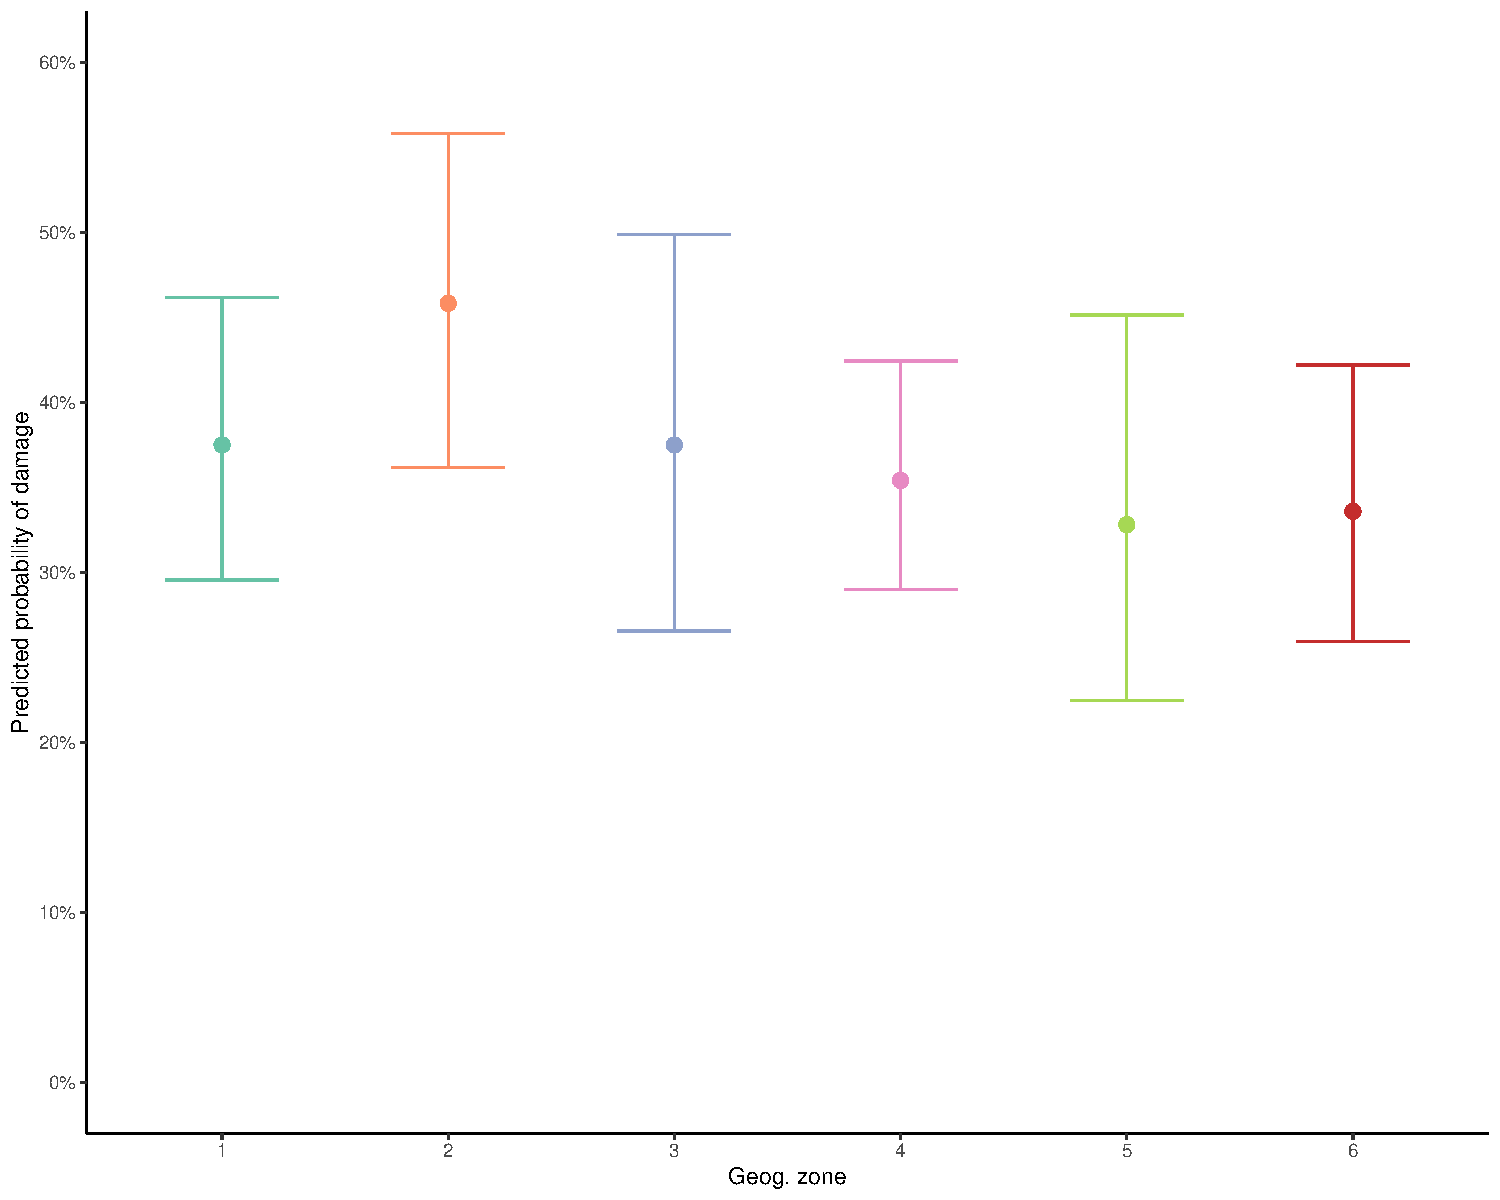
\includegraphics[width=0.5\textwidth]{pred_binom_geog}
	}
	\caption{Predicted values with 95\% confidence intervals for the probability of a sapling being damaged with seed collected from different (a) Sites and (b) aggregated by Geographic Zone.}
	\label{pred_binom}
\end{figure}

\begin{figure}[H]
\centering
	\subfloat[]{
		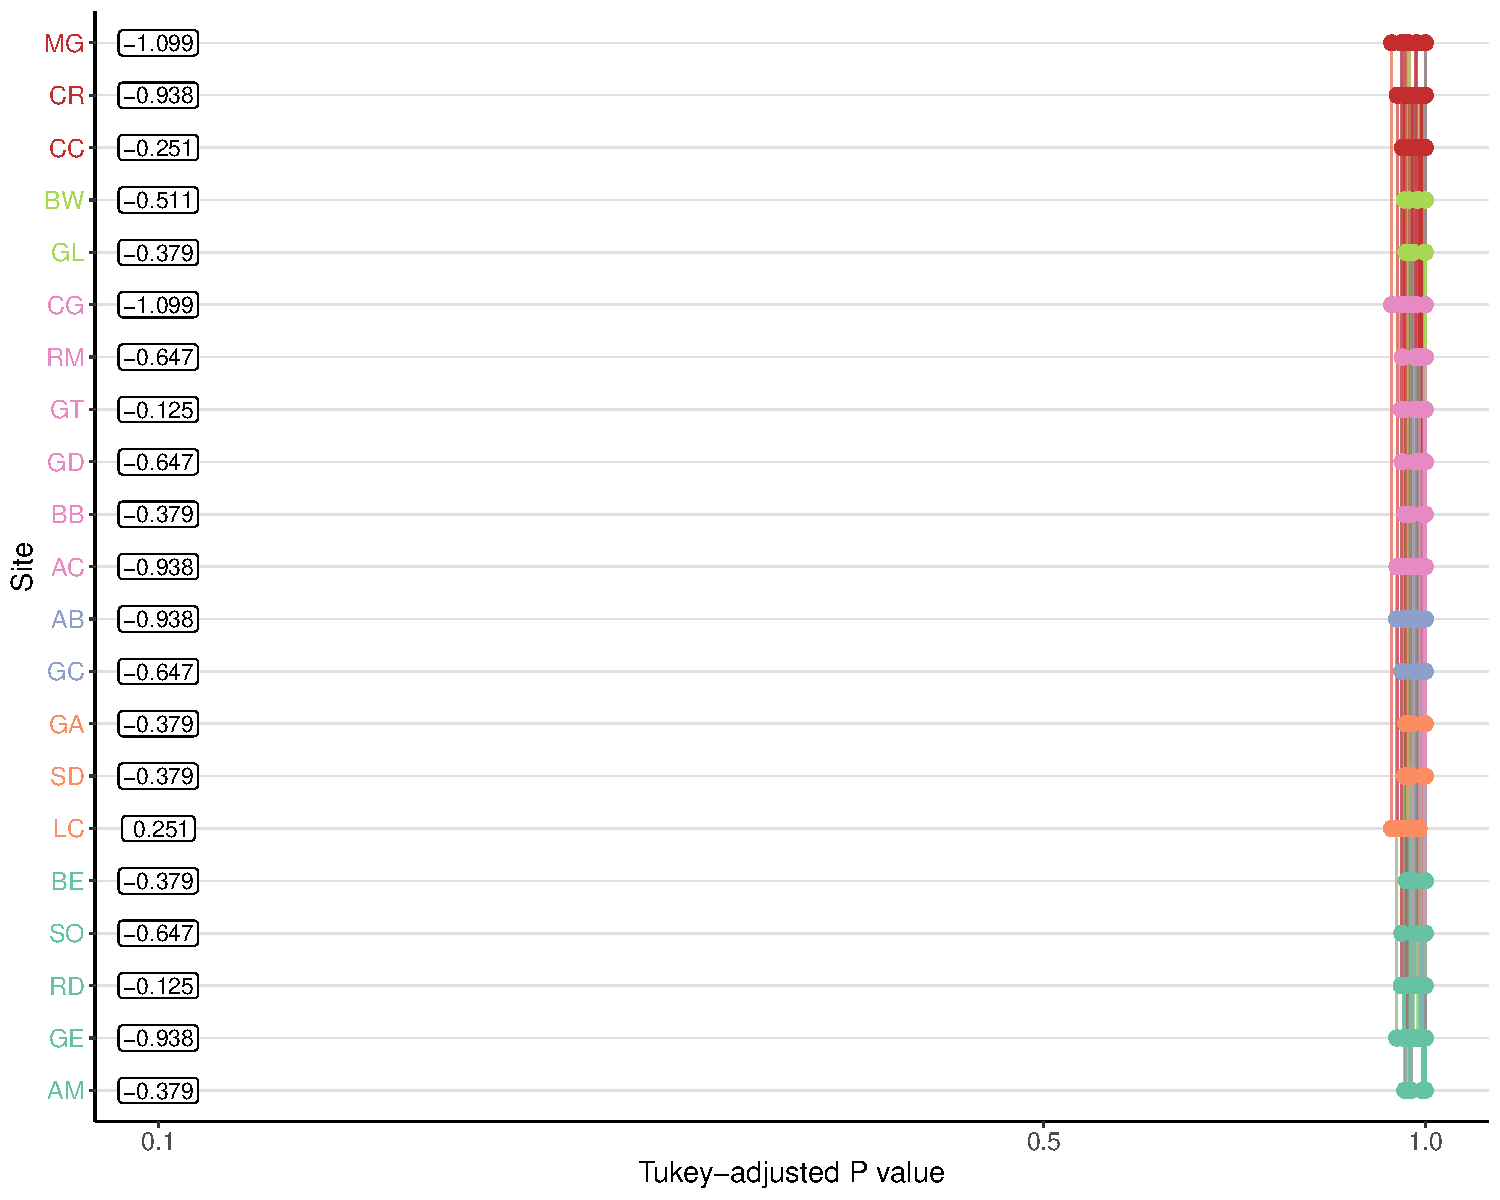
\includegraphics[width=0.5\textwidth]{margin_binom_site}
	}
	\subfloat[]{
		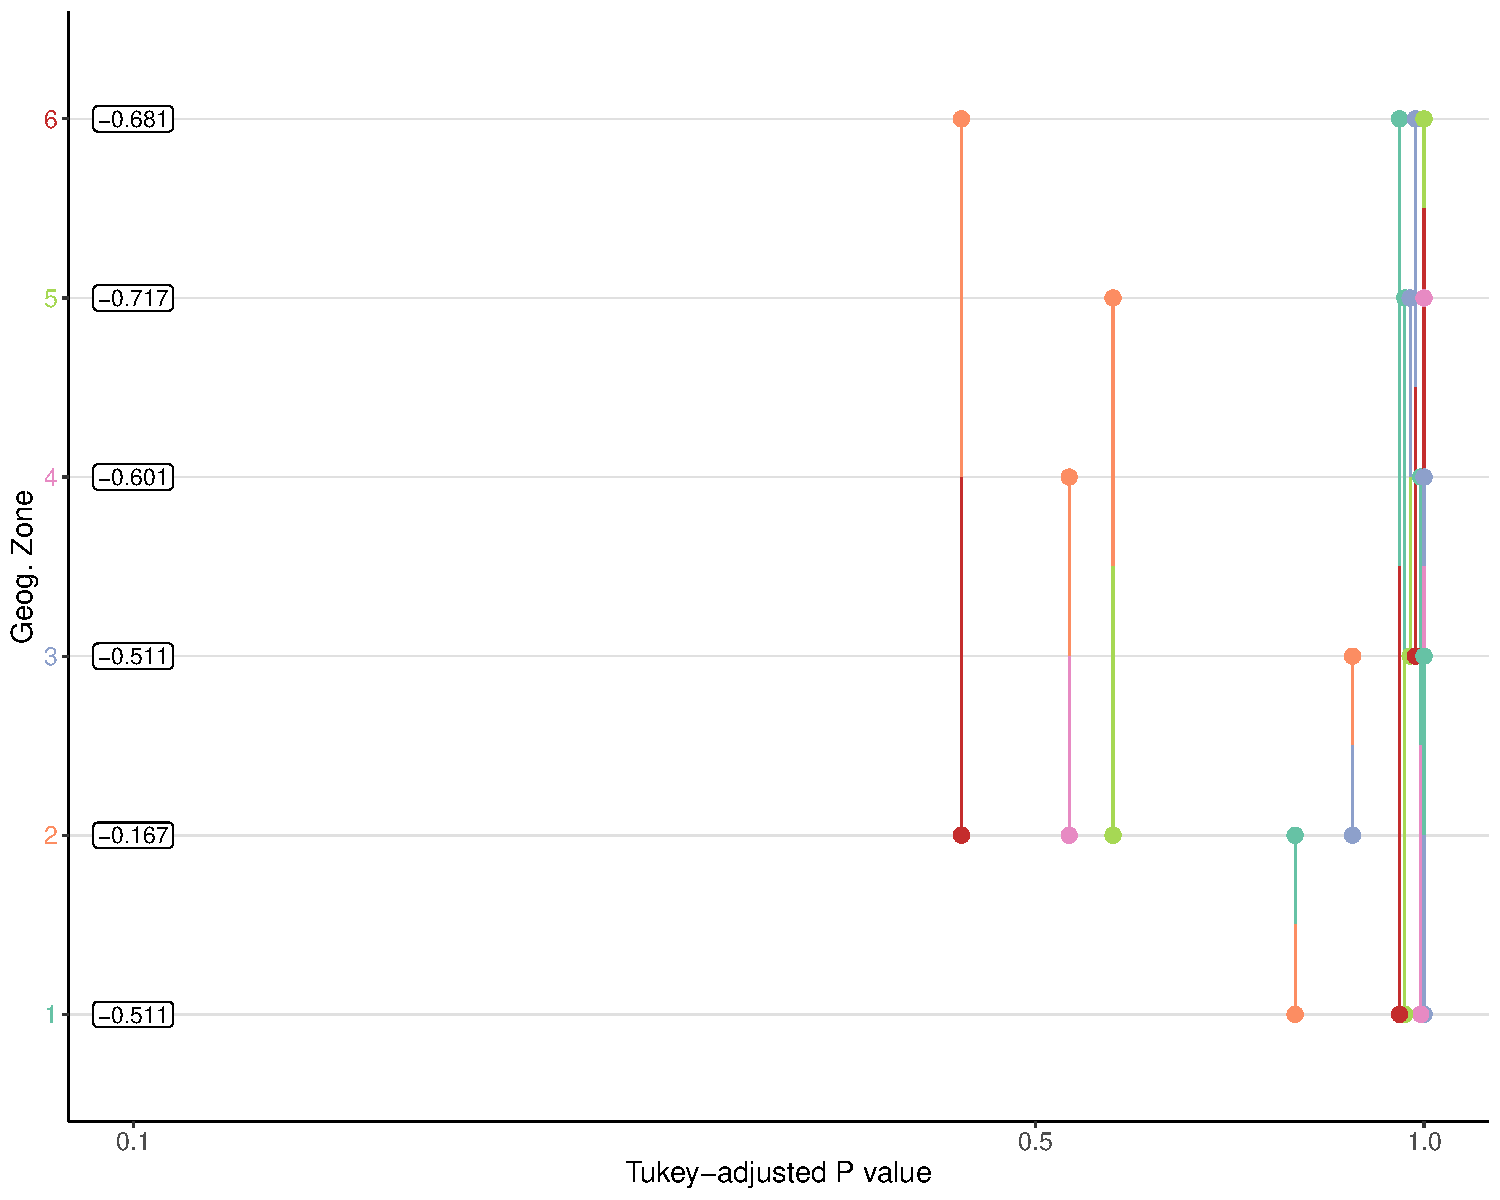
\includegraphics[width=0.5\textwidth]{margin_binom_geog}
	}
	\caption{P-values for Tukey HSD pairwise comparisons of estimated marginal means between (a) Site and (b) Geographic Zone).}
	\label{binom_margin}
\end{figure}


% Table created by stargazer v.5.2.2 by Marek Hlavac, Harvard University. E-mail: hlavac at fas.harvard.edu
% Date and time: Wed, Aug 07, 2019 - 15:28:06
\begin{table}[!htbp] \centering 
  \caption{Model comparison of logistic generalised linear mixed effects models predicting the likelihood of a sapling being attacked by \textit{H. abietis}. Models are sorted according to increasing AIC.} 
  \label{binom_comp} 
\begin{tabular}{@{\extracolsep{5pt}} llS[table-format=3.2]S[table-format=3.2]S[table-format=3.2]S[table-format=3.2]} 
\\[-1.8ex]\hline 
\hline \\[-1.8ex] 
{Fixed eff.} & {Random eff.} & {AIC} & {logLik} & {R\textsuperscript{2}\textsubscript{c}} & {R\textsuperscript{2}\textsubscript{m}} \\
\hline \\[-1.8ex] 
NA & NA & 886.953 & -442.476 & 0 & 0 \\ 
NA & Parent & 888.953 & -442.476 & 0 & 0 \\ 
NA & Site & 888.953 & -442.476 & 0 & 0 \\ 
NA & Site / Parent & 890.953 & -442.476 & 0 & 0 \\ 
NA & Geog. Zone / Site / Parent & 892.953 & -442.476 & 0 & 0 \\ 
Geog. Zone & Parent & 894.462 & -440.231 & 0.006 & 0.008 \\ 
Geog. Zone & Site / Parent & 896.462 & -440.231 & 0.006 & 0.008 \\ 
Site & Parent & 910.721 & -433.361 & 0.027 & 0.035 \\ 
Site & Geog. Zone & 910.721 & -433.361 & 0.027 & 0.035 \\ 
Site & Geog. Zone + Parent & 912.721 & -433.361 & 0.027 & 0.035 \\ 
Parent & Geog. Zone & 1034.683 & -348.341 & 0.940 & 0.953 \\ 
Parent & Geog. Zone / Site & 1036.683 & -348.341 & 0.941 & 0.954 \\ 
\hline \\[-1.8ex] 
\end{tabular} 
\end{table} 


The fixed effect of Site was weak as a predictor of likelihood of \textit{H. abietis} damage. In a model using seed population as a fixed effect and Parent as a random intercept effect, seed population only accounted for 2.7\% (R\textsuperscript{2}\textsubscript{m} of the variation in the probability that a sapling would be initially damaged by \textit{H. abietis}. According to the best fitting model with Site as a fixed effect, saplings from Beinn Eighe (BE) had a greater chance of being initially damaged than others (Figure \ref{pred_binom}a), however, these predicted values were not significantly different from other Sites according to a comparison of marginal means (Figure \ref{binom_margin}a).

\subsubsection*{Non-zero damage model}

The second part of the hurdle model explored variation in the area of sapling bark damaged by \textit{H. abietis}, for those saplings which were initially damaged. The most parsimonious model according to AIC included the fixed effect of Geographic Zone and the random effect of Site to account for pseudo-replication in seed origin. This model explained 5.6\% (R\textsuperscript{2}\textsubscript{m} of the variance in sapling bark area damaged. This model was of better quality than a null model and multiple random effects models. As with the logistic models, models with Parent as a fixed effect explained more variance in damaged bark area, but a pairwise comparison of estimated marginal means showed that no families differed significantly from each other, indicating that the model is over-fitted. The Parent BE4, collected from Beinn Eighe contrasted weakly with a number of families from more southerly Sites, but none significantly (P\textless{}0.05) (Figure \ref{lmer_margin_family}).

In a pairwise comparison of estimated marginal means of Geographic Zones for the best-fitting model, Geographic Zone 1 differed significantly from Zones 4 and 6, and weakly with Zone 5. At the Site level, Rhiddoroch (RD) differed from Glen Derry and Crannach, both populations in the southern part of the study region. Geographic Zone one had a higher predicted damaged bark area according to the best fitting model (Figure \ref{pred_lmer}b). AC and CC had a higher predicted damaged bark area than other Sites.

\begin{figure}[H]
\centering
	\subfloat[]{
		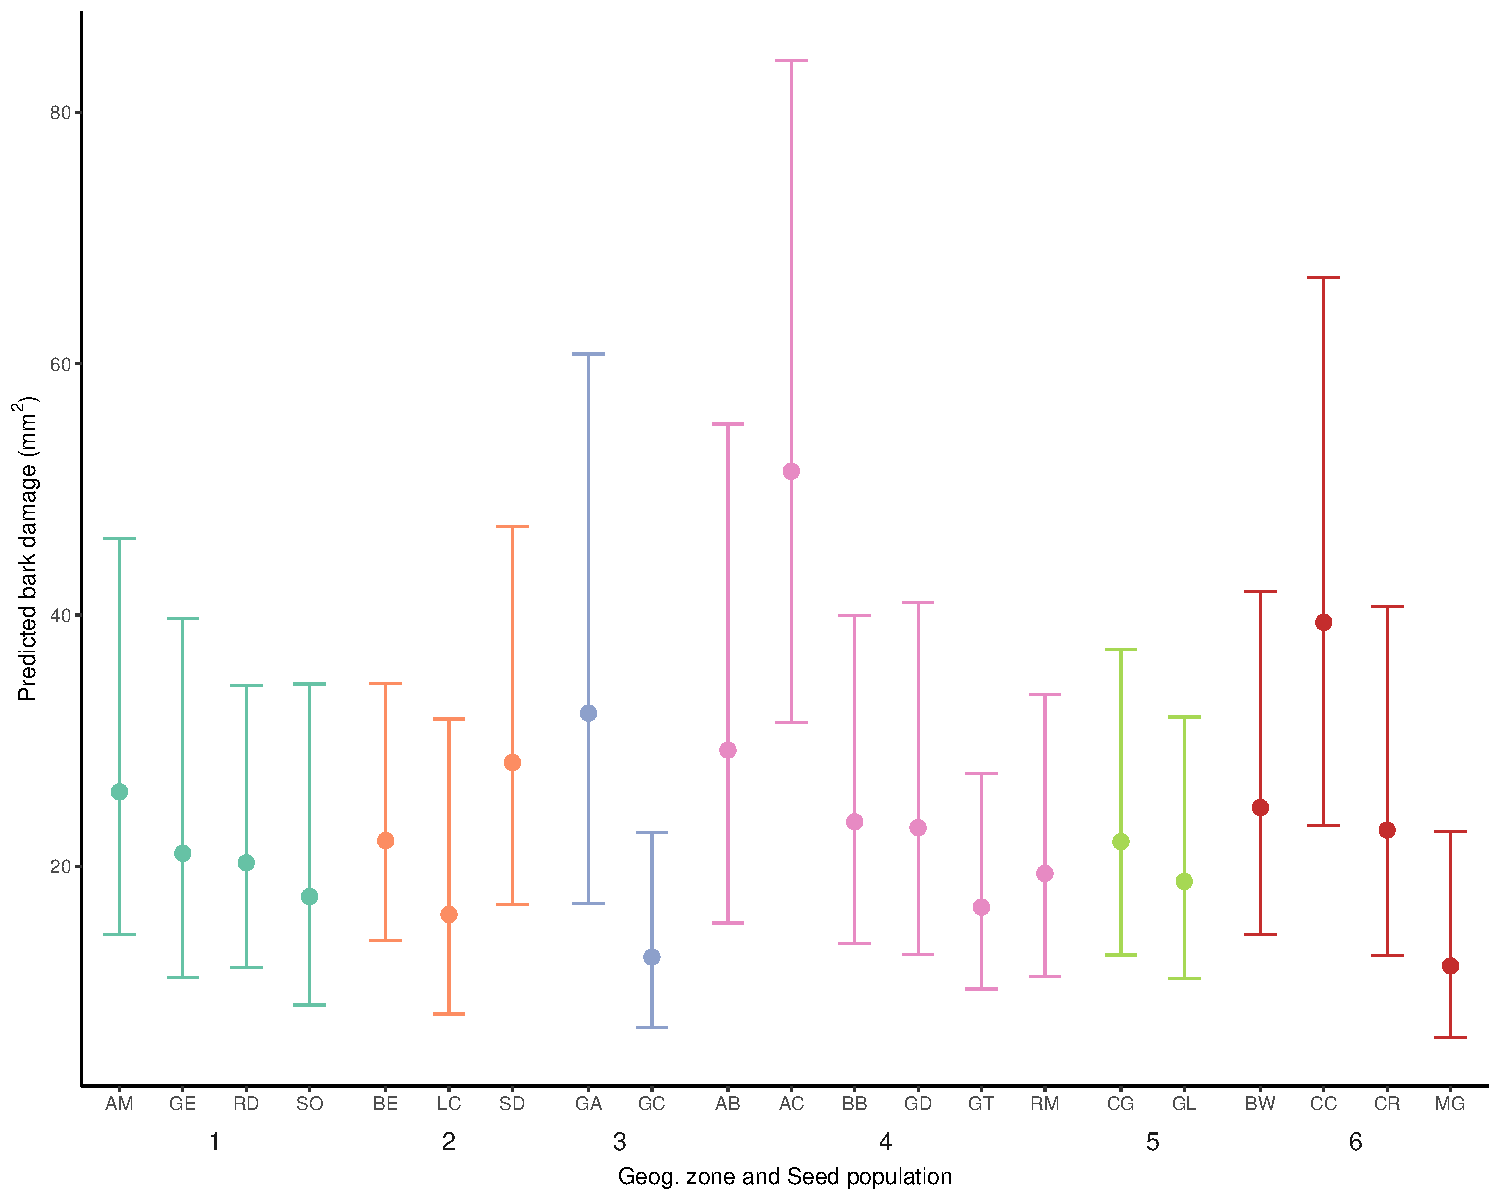
\includegraphics[width=0.5\textwidth]{pred_lmer_site}
	}
	\subfloat[]{
		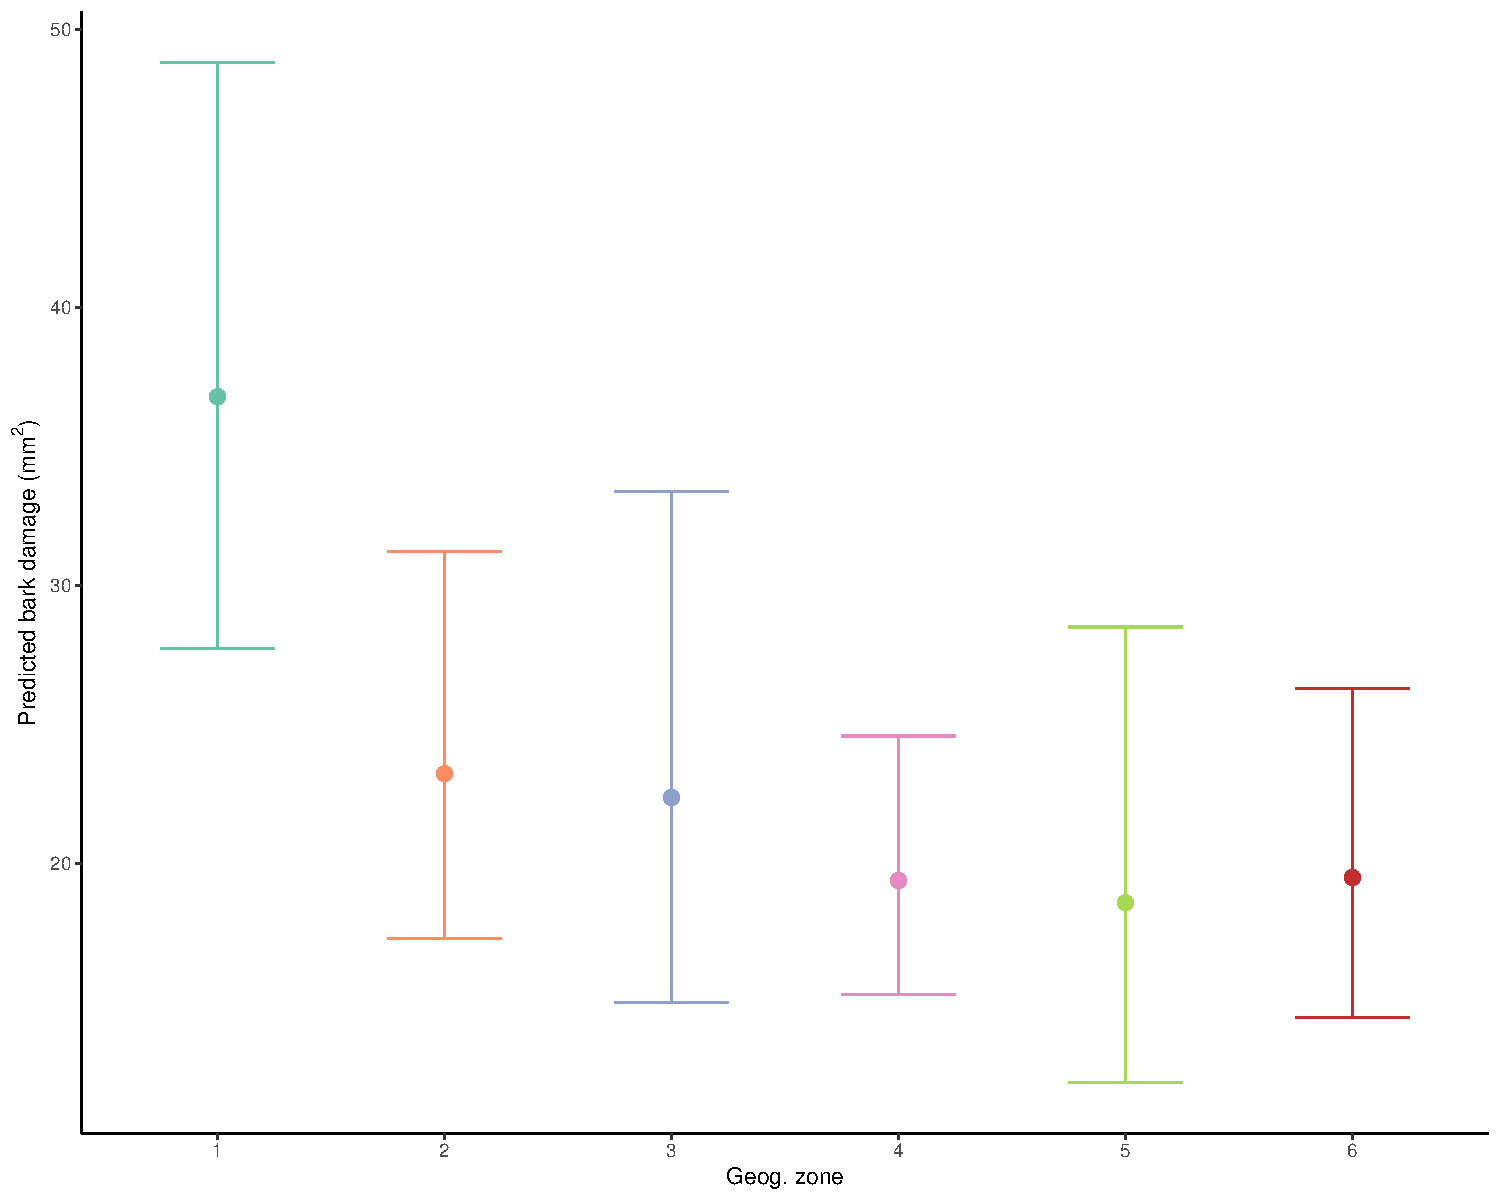
\includegraphics[width=0.5\textwidth]{pred_lmer_geog}
	}
	\caption{Predicted values of mm\textsuperscript{2} for saplings with seed collected from different Geographic Zones.}
	\label{pred_lmer}
\end{figure}

\begin{figure}[H]
\centering
	\subfloat[]{
		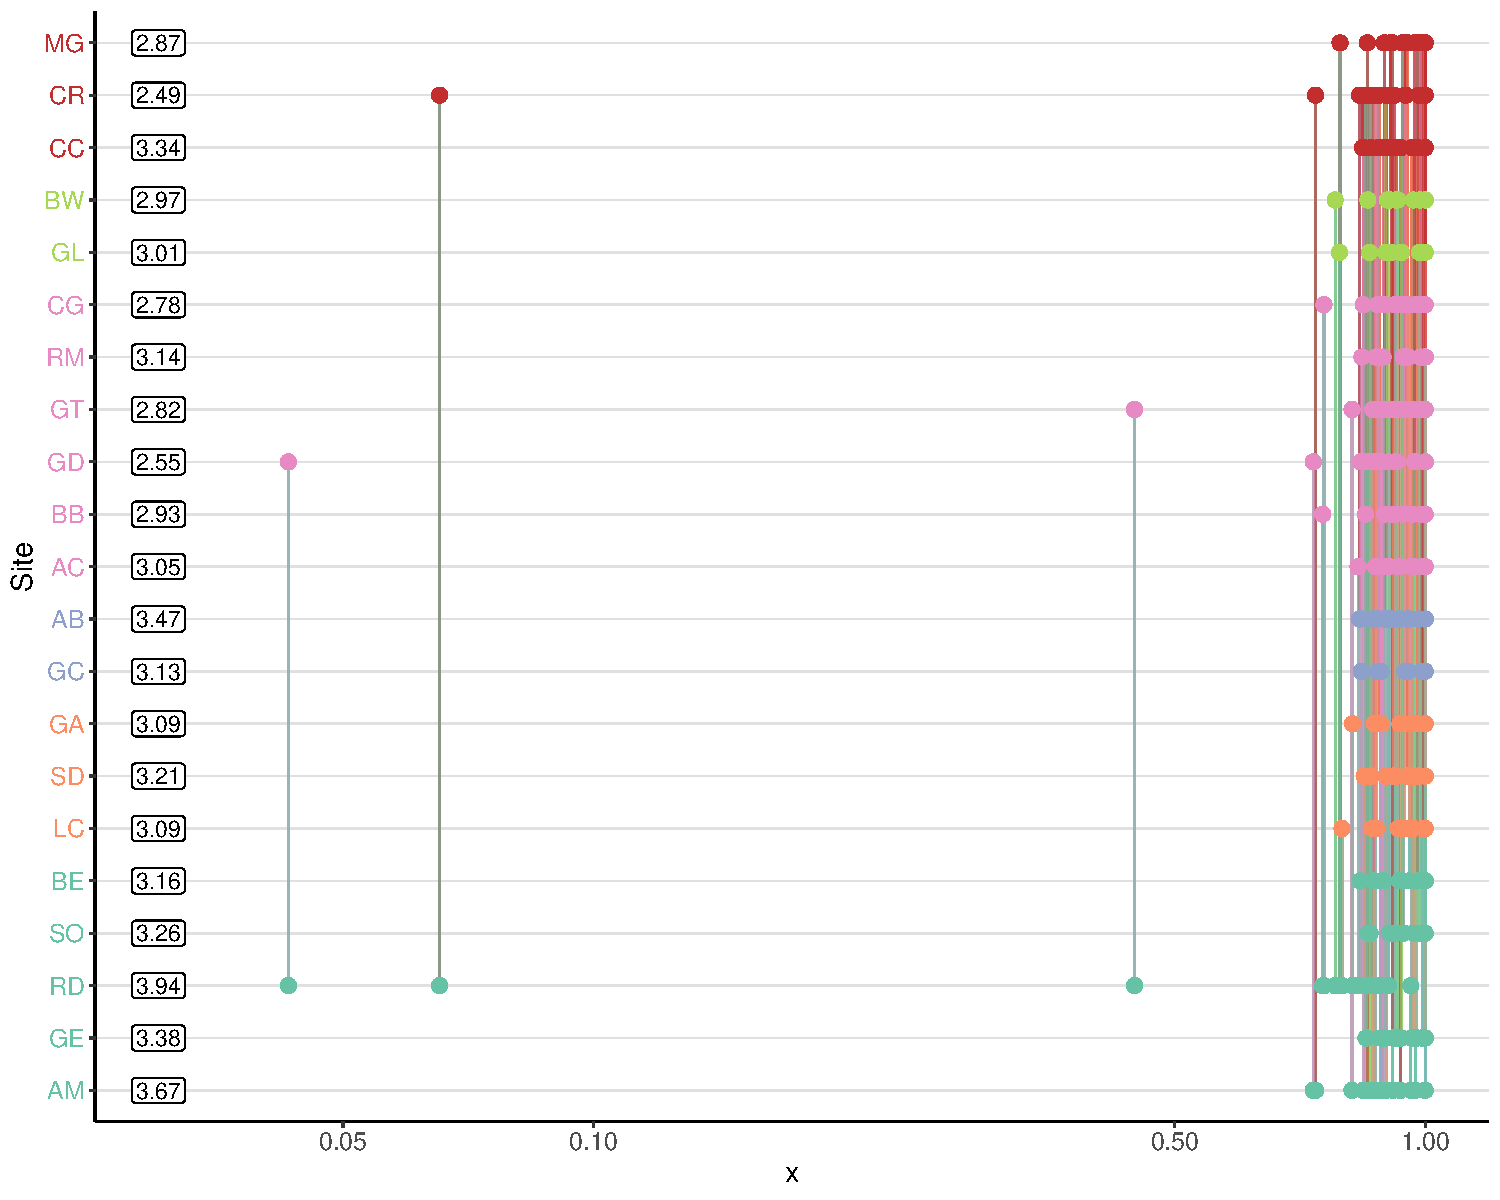
\includegraphics[width=0.5\textwidth]{margin_lmer_site}
	}
	\subfloat[]{
		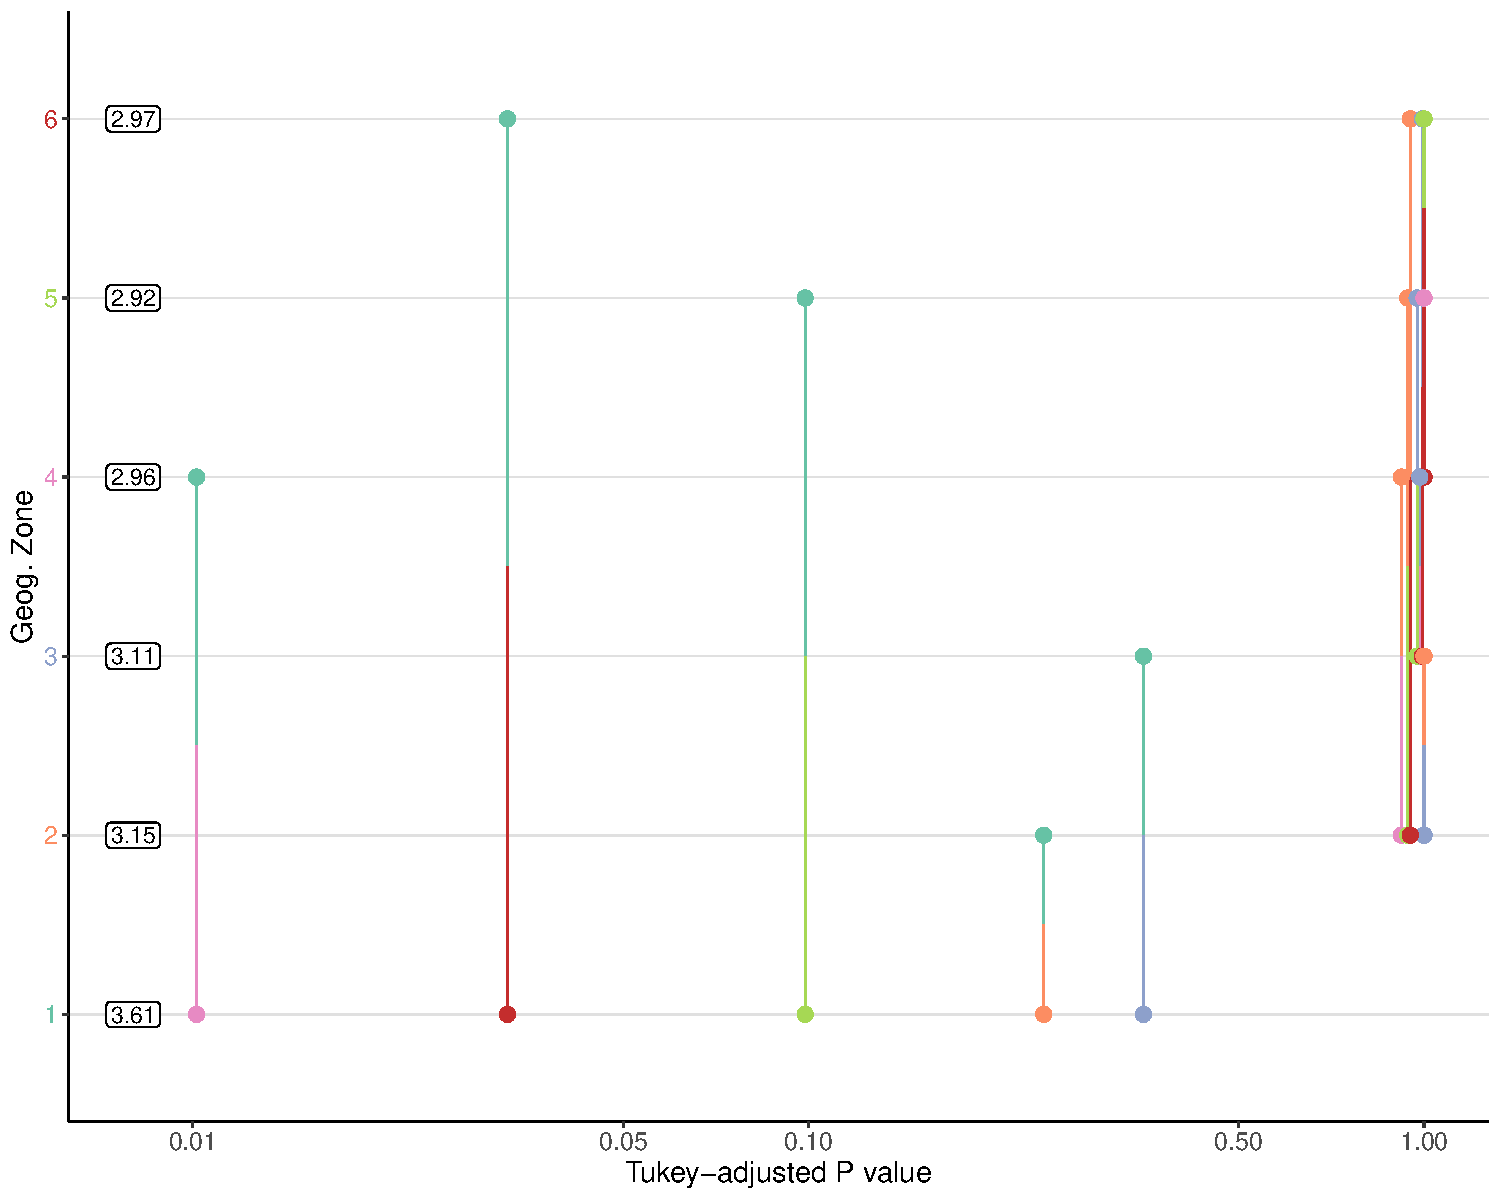
\includegraphics[width=0.5\textwidth]{margin_lmer_geog}
	}
	\caption{P-values for Tukey HSD pairwise comparisons of estimated marginal means between (a) Site and (b) Geographic Zone).}
	\label{lmer_margin}
\end{figure}

\begin{figure}[H]
\centering
	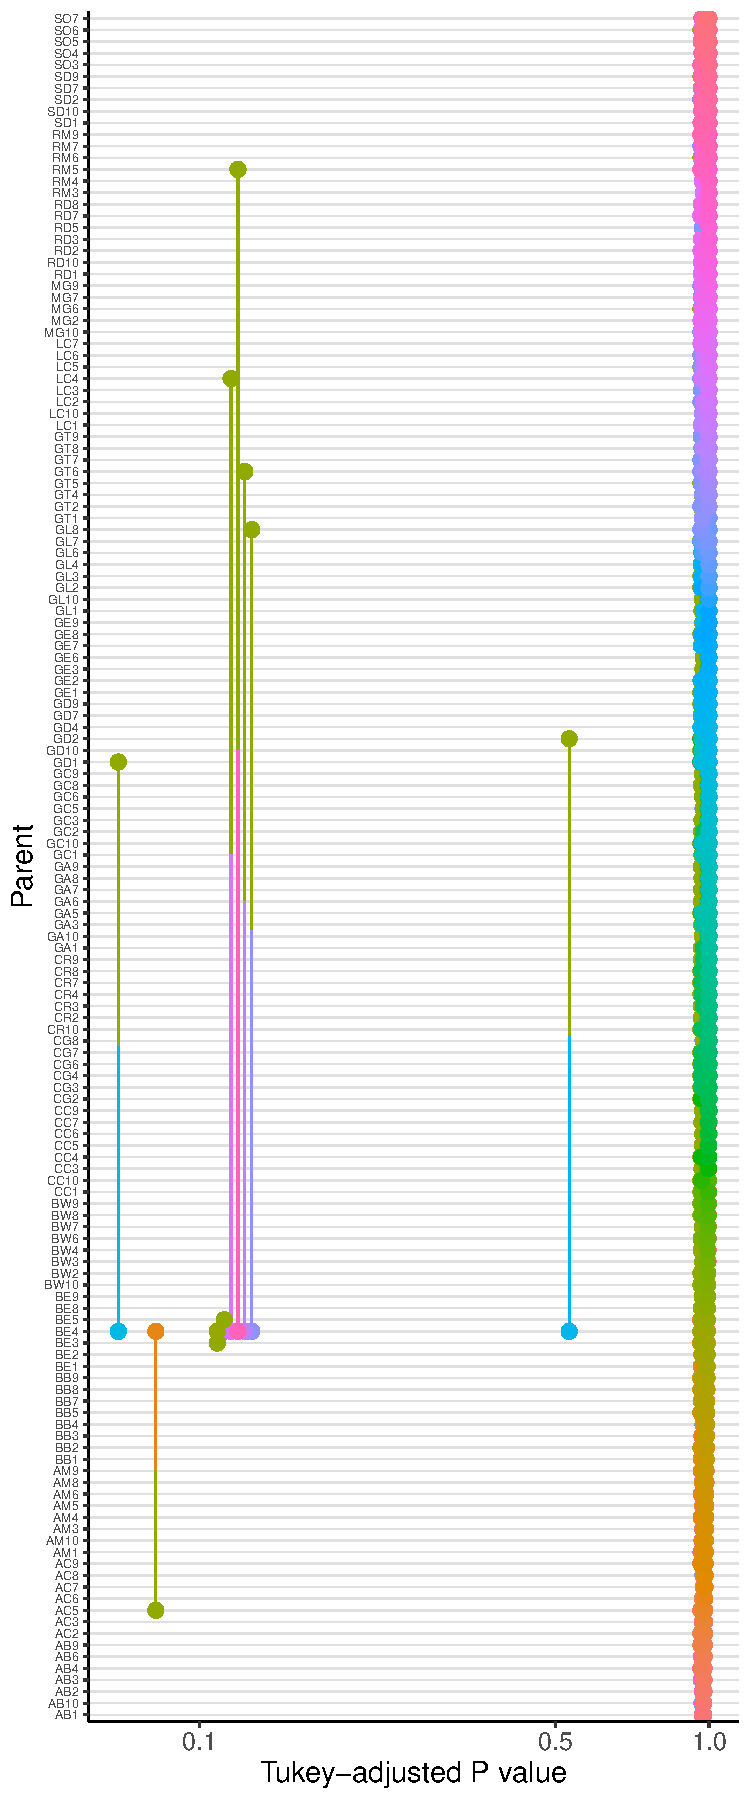
\includegraphics[width=0.6\textwidth]{margin_lmer_family}
	\caption{P-values for Tukey HSD pairwise comparisons of estimated marginal means between sapling Parent groups.}
	\label{lmer_margin_family}
\end{figure}


% Table created by stargazer v.5.2.2 by Marek Hlavac, Harvard University. E-mail: hlavac at fas.harvard.edu
% Date and time: Wed, Aug 07, 2019 - 15:28:12
\begin{table}[!htbp] \centering 
  \caption{Model comparison of general linear mixed effects models predicting the damaged bark area of a sapling, for those saplings which have been initially damaged. Models are sorted according to increasing AIC.} 
  \label{lmer_comp} 
\begin{tabular}{@{\extracolsep{5pt}} llS[table-format=3.2]S[table-format=3.2]S[table-format=3.2]S[table-format=3.2]} 
\\[-1.8ex]\hline 
\hline \\[-1.8ex] 
{Fixed eff.} & {Random eff.} & {AIC} & {logLik} & {R\textsuperscript{2}\textsubscript{c}} & {R\textsuperscript{2}\textsubscript{m}} \\
\hline \\[-1.8ex] 
Geog. Zone & Site & 719.471 & -351.735 & 0.056 & 0.056 \\ 
NA & NA & 721.787 & -358.893 & 0 & 0 \\ 
NA & Geog. Zone / Site & 722.193 & -357.096 & 0.033 & 0 \\ 
NA & Site / Parent & 724.929 & -358.464 & 0.026 & 0 \\ 
Site & Geog. Zone & 736.127 & -345.063 & 0.106 & 0.106 \\ 
Site & Parent & 736.127 & -345.063 & 0.106 & 0.106 \\ 
Site & Geog. Zone + Parent & 738.127 & -345.063 & 0.106 & 0.106 \\ 
Parent & Geog. Zone & 810.131 & -256.066 & 0.565 & 0.565 \\ 
Parent & Geog. Zone / Site & 812.131 & -256.066 & 0.565 & 0.565 \\ 
Geog. Zone & Site / Parent &  &  & 0.056 & 0.056 \\ 
\hline \\[-1.8ex] 
\end{tabular} 
\end{table} 


\subsection*{Population level spatial patterns}

There was a weak but significant positive effect of latitude on the total bark area damaged by \textit{H. abietis} (Z = 3.249(1, 248), p =  \textless{}0.005, R\textsuperscript{2}\textsubscript{m} = 0.041), when the nested random effects of seed collection Site and family were accounted for (Figure \ref{latitude}). In a similar model, there was no effect of longitude on bark area damaged (Z = -1.377(1, 248), p = 0.168, R\textsuperscript{2}\textsubscript{m} = 0.009).  

\begin{figure}[H]
	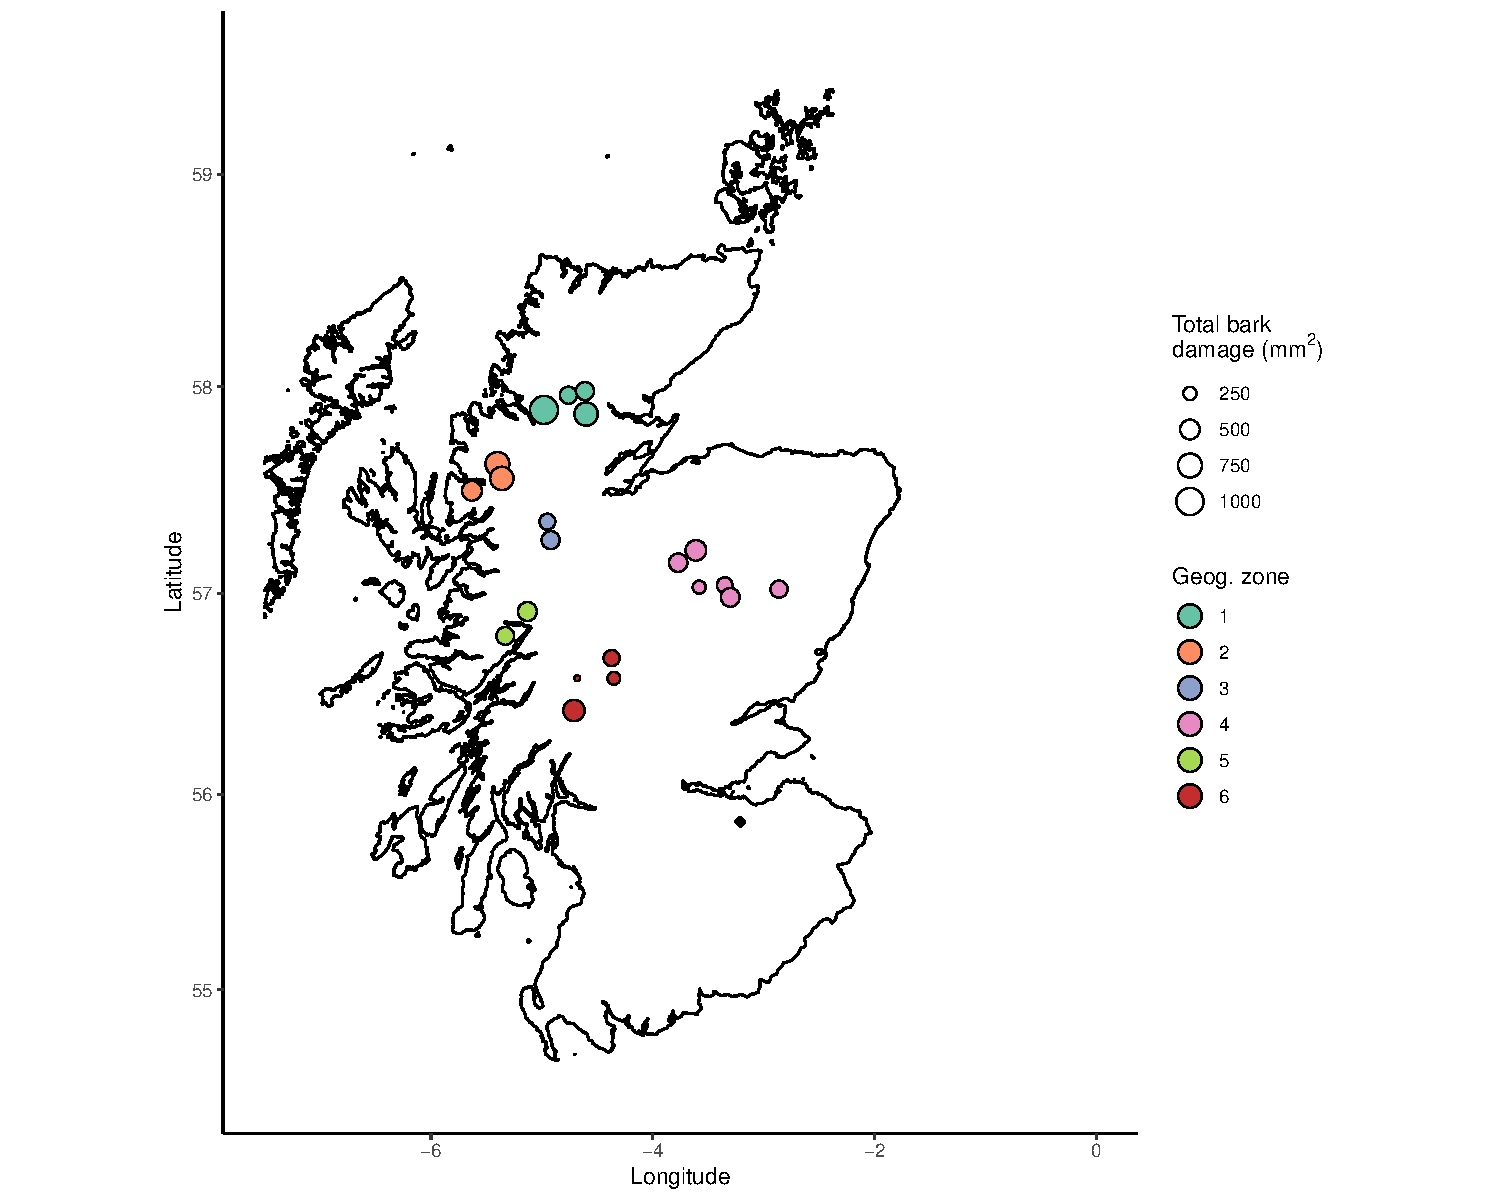
\includegraphics[width=\textwidth]{bubble_map}	
	\caption{Map of study Sites with bubbles coloured according to Geographic Zone and relatively sized according to the total bark area damaged for all 32 saplings per Site.}
	\label{bubble_map}
\end{figure}

\begin{figure}[H]
	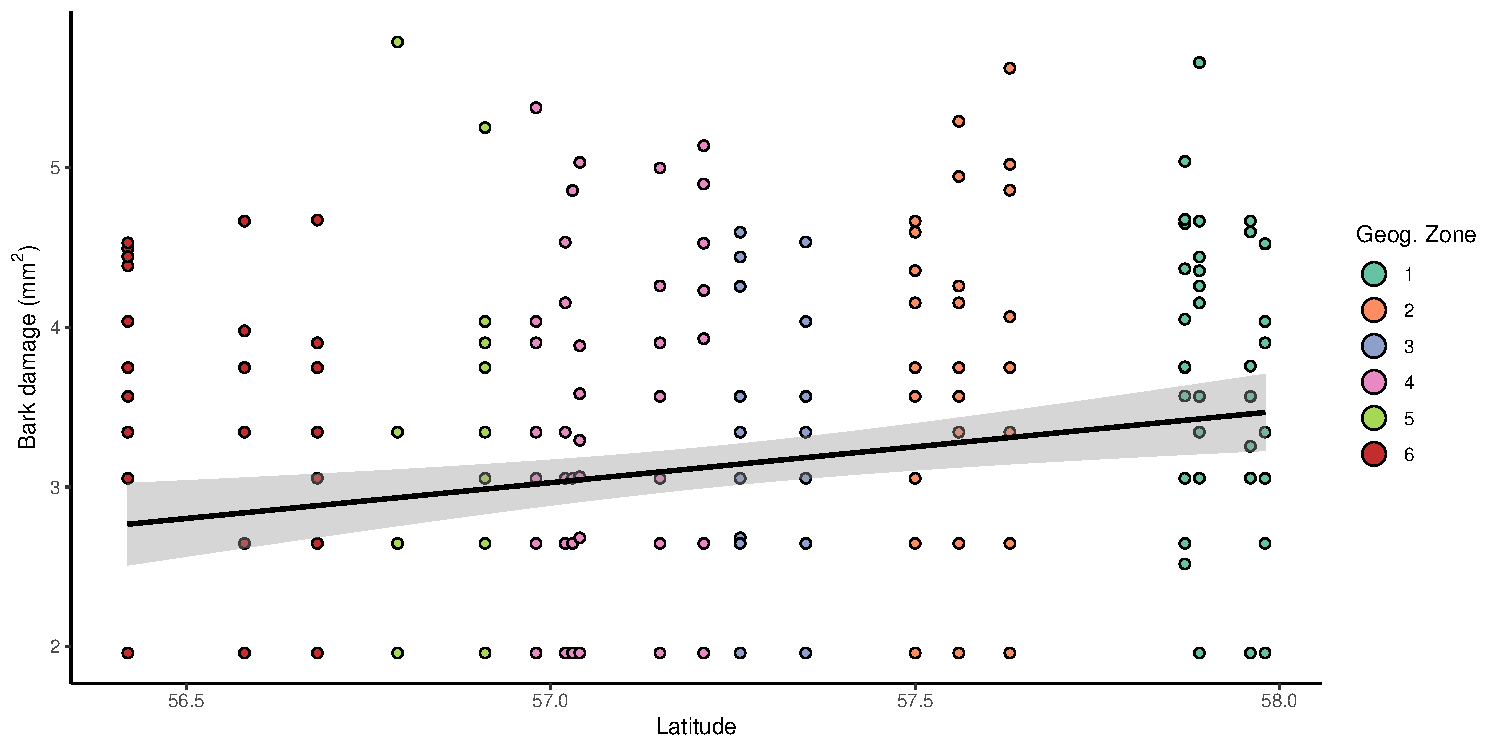
\includegraphics[width=\textwidth]{latitude}
	\caption{Relationship between bark area damaged and latitude of sapling population, for those saplings which were damaged. Each point is an individual sapling. Points are coloured by Geographic Zone. The linear model fit (black line with grey 95\% confidence interval) shows a weak positive trend.}
	\label{latitude}
\end{figure}

\begin{figure}[H]
	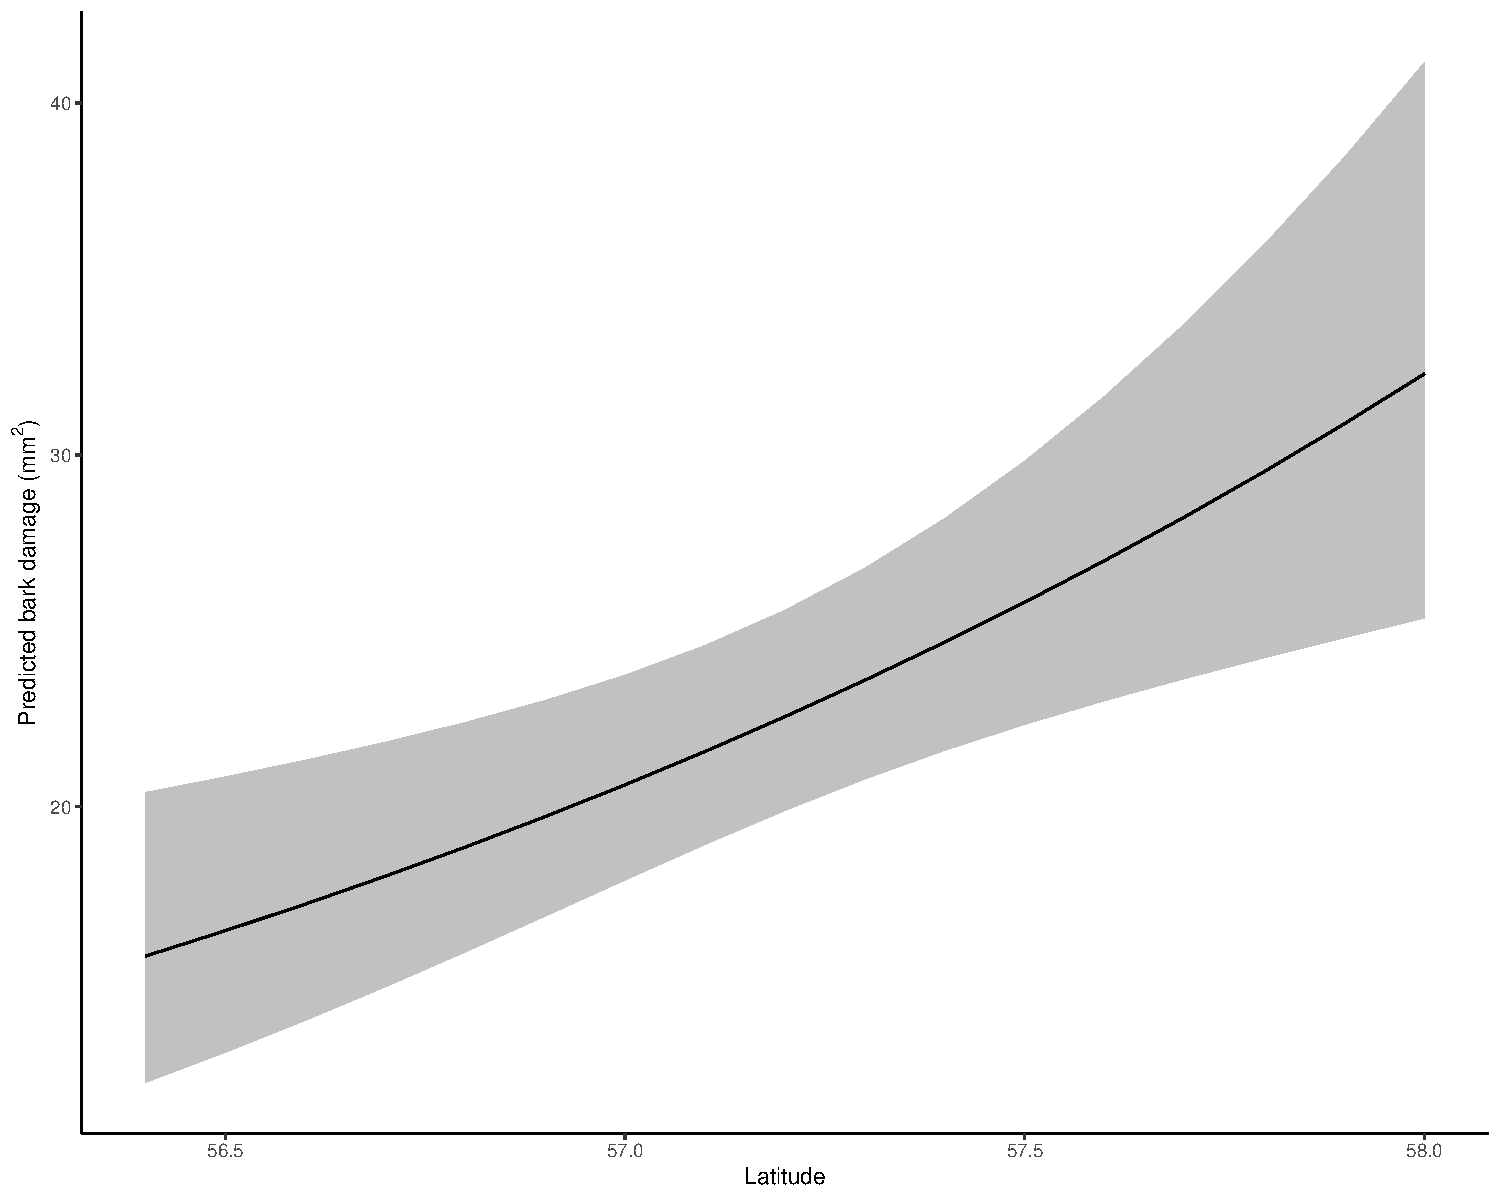
\includegraphics[width=\textwidth]{pred_lat}
	\caption{Predicted values with 95\% confidence interval for the bark area damaged on a sapling with seed  collected at different latitudes.}
\end{figure}

\section*{Discussion}

The model selection process determined that there was an effect of Geographic Zone on the area of weevil damage found on damaged saplings and a possible weak effect of Site, but could not account for variation in the probability that a sapling became damaged initially. Linear Mixed Effects models demonstrated that there was a general latitudinal effect on sapling damaged area. Saplings with Parents at higher latitudes typically experienced higher levels of damage, but this had a much weaker effect than population or Geographic Zone itself. Within Site variability among Parents was high and diluted the effects of Geographic Zone and Site. This is expected given the high gene flow between populations \citep{Donnelly2018}. Nevertheless, some clear variation was observed between groups.

In this study we identified weak but significant differences between \textit{P. sylvestris} populations in their susceptibility to \textit{H. abietis} attack. It appears that a weak latitudinal pattern may be driving these differences. It may be that historical exposure to \textit{H. abietis} in more southerly populations has driven adaptation to develop defensive structures to deter bark feeding insects. Studies on the distribution and life cycle of \textit{H. abietis} have shown that life cycle length is strongly linked with mean temperature in the summer months, with higher temperatures leading to a short life cycle and therefore higher numbers of pine weevils where infestations occur \citep{Leather1999}. \textit{H. abietis} abundance reduces with latitude in Scotland \citep{Barredo2015}. Historically, \textit{H. abietis} populations at high latitudes and in the west of Scotland have been low \citep{Leather1999}, due to lower temperatures \citep{Wainhouse2014}. The latitudinal effect may therefore be a result of adaptation to resist \textit{H. abietis} damage. Additionally, phenological variation in latitudinal populations may lead to VOC concentrations varying between saplings at the same time of year in the common garden, making some saplings more desirable than others \citep{Guenther1997}. The data collection for this study took place in June, approximately between the two seasonal peaks of \textit{H. abietis} activity. Other studies have shown that the growing season of \textit{P. sylvestris} from higher latitudes starts later in the year \citep{Salmela2013}, leading to a lower concentration of VOC stored in bark resin when our study was conducted, potentially making these saplings more attractive than those from southerly populations to \textit{H. abietis}. \citet{Yazdani1985} found that \textit{P. sylvestris} individuals in Sweden varied in the composition of monoterpenes found in oleoresin, with northern populations containing lower limonene, lower $\Beta$-pinene and higher $\Delta$3-carene. \citet{Nordlander1990} found that \textit{H. abietis} limonene inhibits the efficiency of $\alpha$-pinene, a chemical which is known to attract \textit{H. abietis}, meaning more northerly \textit{P. sylvestris} populations may be more attractive to \textit{H. abietis}.

\textit{P. sylvestris} needles and bark have resin canals which act to deter herbivores. While it has not been explicitly tested for \textit{H abietis}, other studies involving similar bark feeding insects have found a negative correlation between resin canal density and feeding behaviour on coniferous tree species. \citet{Boucher2001} found that the white pine weevil \textit{Pissodes strobi} was discouraged from eating the needles of four different pine species with higher resin canal concentration and cuticle thickness. \citet{Donnelly2016} found that for a subset of the same seed population Sites studied here, that resin canal density in needles varied with longitude and between Sites, but did not test latitudinal variation. They suggested that resin canal density may be linked to water stress, as it plays a role in water regulation \citep{Farrell1991}. Interestingly, this study found no complementary correlation between longitude and damage by \textit{H. abietis}. 

As climate change increases average temperatures at high latitudes, there is the possibility that \textit{H. abietis} and other bark feeding insect herbivores will become more present at high latitudes \citep{Inward2012}. This study shows that there is a potential risk to both naturally occurring and planted forests with seed stock gathered from high latitudes as these varieties appear more susceptible to \textit{H. abietis} attack. We suggest that future work seeks to identify variation in VOC concentration and composition within \textit{P. sylvestris} populations to identify at risk populations to allow the creation of prioritised conservation management strategies as climate change progresses.

\section*{Conclusion}

This study sought to test whether adaptive variation for resistance to the large pine weevil (\textit{Hylobius abietis}) existed in genetically distinct populations of scots pine (\textit{Pinus sylvestris}) in Caledonian remnant forest patches in Scotland. A weak positive effect of latitude of seed collection Site was found in the damaged area of sapling bark, suggesting that more southerly populations may be less attractive to \textit{H. abietis} attack. No relationship was found between Site and probability of a sapling being initially damaged. Variation exists between Geographic Zones and between Sites with regards to resistance to continued \textit{H. abietis} attack. The conclusions of this study suggest that under warming temperatures as a result of anthropogenic climate change, there is a conservation concern for less-resistant Caledonian remnant forest patches as \textit{H. abietis} populations may increase, leading to higher mortality of saplings, leading to changes in ecosystem structure. It is suggested that further studies should investigate bark morphological and physiological variation amongst these natural populations of \textit{P. sylvestris}, with particular attention to variation in Volatile Organic Compounds (VOCs) emitted when bark is damaged as a defensive response in young saplings, to understand the underlying mechanism driving differences between these genetically distinct populations.

\bibliography{weevils}

%-----------------------------------------------
\end{document}
%-----------------------------------------------
